\chapter{CRUD WITH SPRING ANGULAR}

\section{Memulai}

Untuk membangun \textit{project} dengan Spring dan AngularJS, lebih mudahnya kita mengawali dengan membuat kerangka dari \url{http://start.spring.io}. 

Beberapa pustaka yang perlu kita sertakan adalah sebagai berikut :

\begin{itemize}
	\item JPA. Yang nantinya kita butuhkan untuk memudahkan melakukan operasi manipulasi basis data.
	\item Rest Repositories. Ini digunakan \textit{backend service} mengirimkan pesan atau data ke \textit{front-end service} Angular.
	\item Security. Ini adalah paket atau modul yang disediakan \textit{Framework} Spring untuk menjaga / mengotorisasi akses \textit{user}.
	\item Thymeleaf. Digunakan untuk melakukan \textit{templating} halaman \texttt{html}.
	\item Web. Digunakan untuk implementasi MVC pada aplikasi web yang kita bangun.
	\item PostgreSQL. Digunakan sebagai \textit{driver} basis data yang menghubungkan Java dengan basis data postgresql.
	\item Lombok. Digunakan untuk menjadikan kode yang kita buat lebih bersih.
\end{itemize}

Pada halaman \url{start.spring.io} akan terlihat seperti gambar \ref{fig:generate-package-angular} berikut :

\begin{figure}[H]
	\centering
	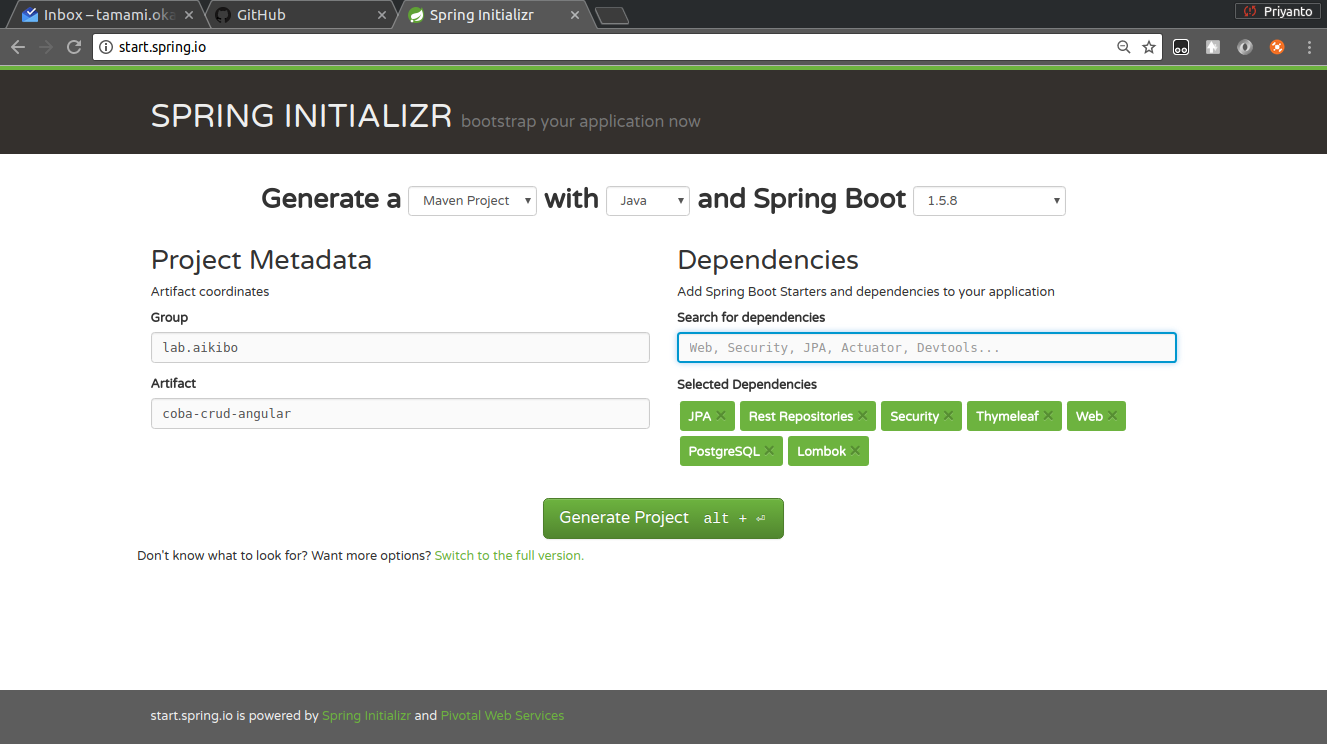
\includegraphics[width=1\textwidth]{./resources/016-generate-package-angular}
	\caption{\textit{Generate Project} Untuk Spring Angular}
	\label{fig:generate-package-angular}
\end{figure}
	
Selanjutnya kita ubah terlebih dahulu \textit{file} \texttt{application.properties} dengan konfigurasi koneksi basis data, karena kita telah menambahkan Spring JPA dalam konfigurasi Maven kita. Berikut adalah isi dari \textit{file} konfigurasi \texttt{application.properties} :

\begin{lstlisting}
spring.datasource.url = jdbc:postgresql://localhost:5432/phb
spring.datasource.username = dev
spring.datasource.password = rahasia
spring.datasource.driver-class-name = org.postgresql.Driver

spring.jpa.database-platform=org.hibernate.dialect.PostgreSQL9Dialect

spring.jackson.serialization.indent_output = true
\end{lstlisting}

Setelah pengisian konfigurasi basis data, kita dapat melakukan tes langsung terhadap Spring Security, jalankan dengan Maven dan perhatikan informasi yang muncul di layar seperti pada gambar \ref{fig:default-password} berikut :

\begin{figure}[H]
	\centering
	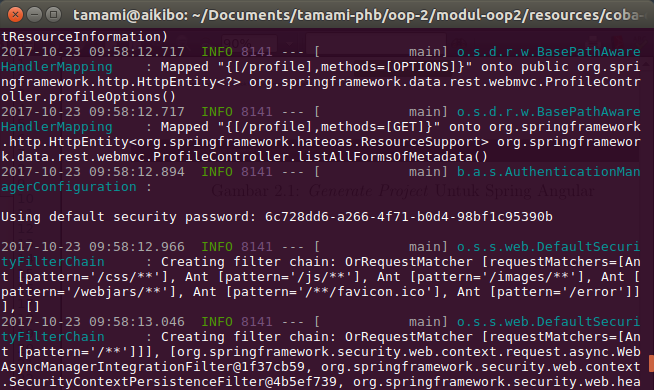
\includegraphics[width=1\textwidth]{./resources/017-default-pass}
	\caption{\textit{Default Password} Spring Security}
	\label{fig:default-password}
\end{figure}

Bukalah \textit{browser} sehingga akan memberikan tampilan seperti gambar \ref{fig:user-ask} berikut ini :

\begin{figure}[H]
	\centering
	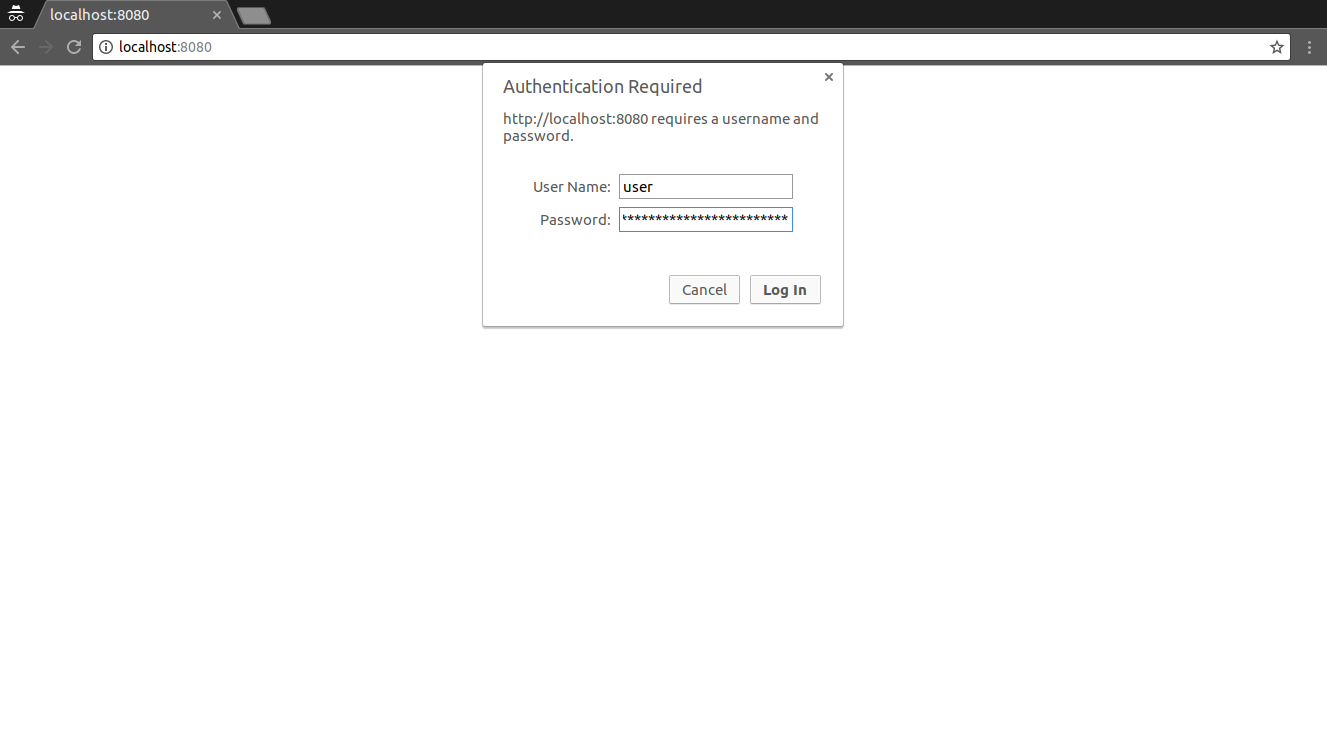
\includegraphics[width=1\textwidth]{./resources/018-user-ask}
	\caption{Isian \textit{User} dan \textit{Password}}
	\label{fig:user-ask}
\end{figure}

Lalu isikan informasi \textit{username} dengan \texttt{user} dan \textit{password} dengan karakter panjang yang diberikan Spring Security di gambar \ref{fig:default-password}.

Setelah itu akan diberikan halaman Rest \textit{default} berupa JSON seperti terlihat pada gambar \ref{fig:index-default} berikut :

\begin{figure}[H]
	\centering
	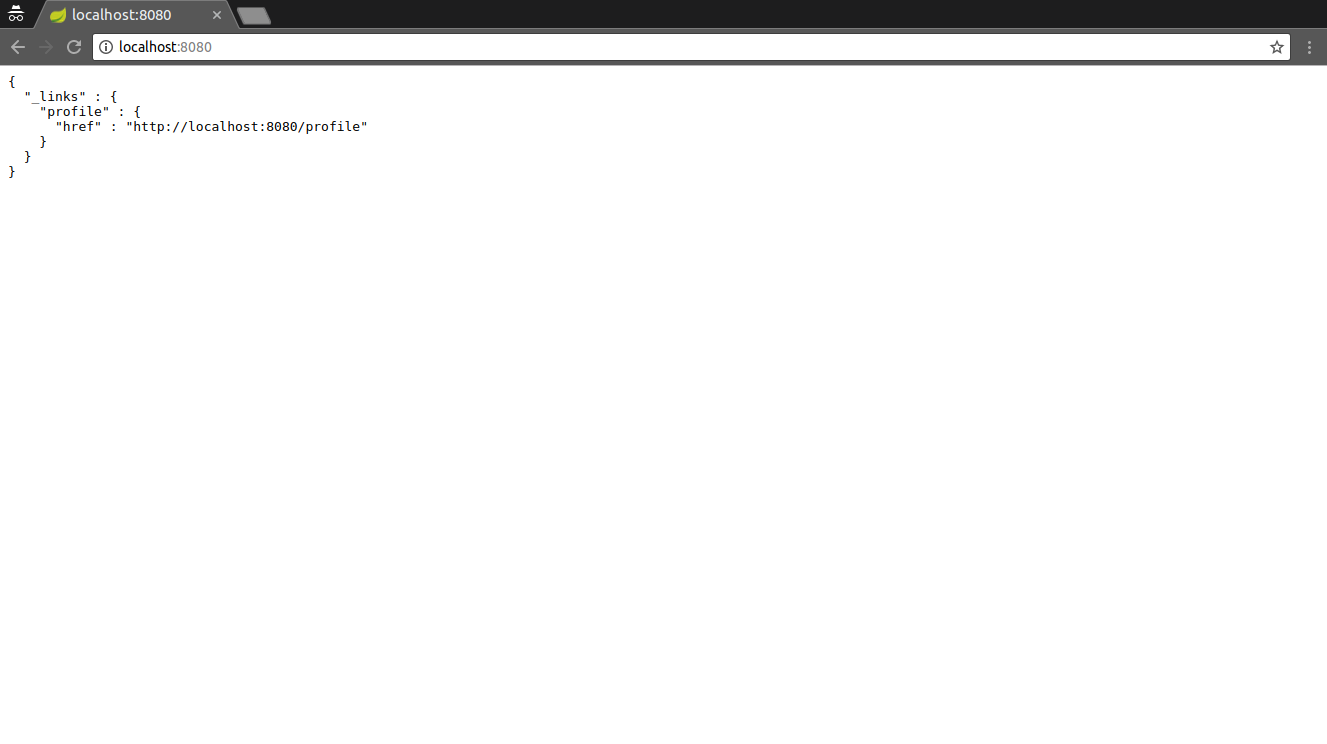
\includegraphics[width=1\textwidth]{./resources/019-default-index}
	\caption{\textit{Default Page} Setelah \textit{Login}}
	\label{fig:index-default}
\end{figure}

Sampai kondisi ini, Spring JPA sudah berhasil terhubung dengan sistem basis data dan \textit{security} telah berjalan dengan baik.

\section{Merubah \textit{Username} dan \textit{Password}}

Lalu bagaimana agar \textit{username} dan \textit{password} dapat kita tentukan sendiri? Berikut adalah langkahnya :

\begin{enumerate}
	\item Menambahkan kelas \texttt{SecurityConfig}. Pada paket \texttt{config} seperti terlihat pada gambar \ref{fig:lokasi-security-config} berikut :
	
	\begin{figure}[H]
		\centering
		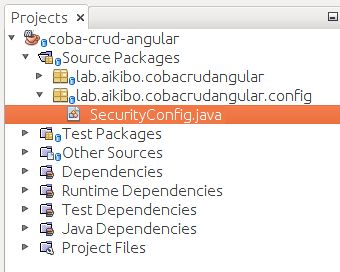
\includegraphics[width=0.5\textwidth]{./resources/021-lokasi-security-config}
		\caption{Lokasi \textit{File} \texttt{SecurityConfig.java}}
		\label{fig:lokasi-security-config}
	\end{figure}
		
	Kode dari kelas \texttt{SecurityConfig} sendiri adalah seperti kode berikut :
	
	\begin{lstlisting}
package lab.aikibo.cobacrudangular.config;

import org.springframework.context.annotation.Configuration;
import org.springframework.security.config.annotation.web.configuration.WebSecurityConfigurerAdapter;
import org.springframework.security.config.annotation.web.servlet.configuration.EnableWebMvcSecurity;
import org.springframework.beans.factory.annotation.Autowired; 
import org.springframework.security.config.annotation.authentication.builders.AuthenticationManagerBuilder;

@Configuration
@EnableWebMvcSecurity
public class SecurityConfig extends WebSecurityConfigurerAdapter {
	
	@Autowired
	public void configureGlobal(AuthenticationManagerBuilder auth) throws Exception {
		auth.inMemoryAuthentication()
			.withUser("tamami")
			.password("rahasia")
			.roles("ADMIN");
	}

}
	\end{lstlisting}
	
	Dengan menambahkan kelas \texttt{SecurityConfig} tersebut, halaman \textit{login} akan berubah bila kita coba jalankan aplikasinya, halaman \textit{login} akan terlihat seperti gambar \ref{fig:custom-login} berikut :
	
	\begin{figure}[H]
		\centering
		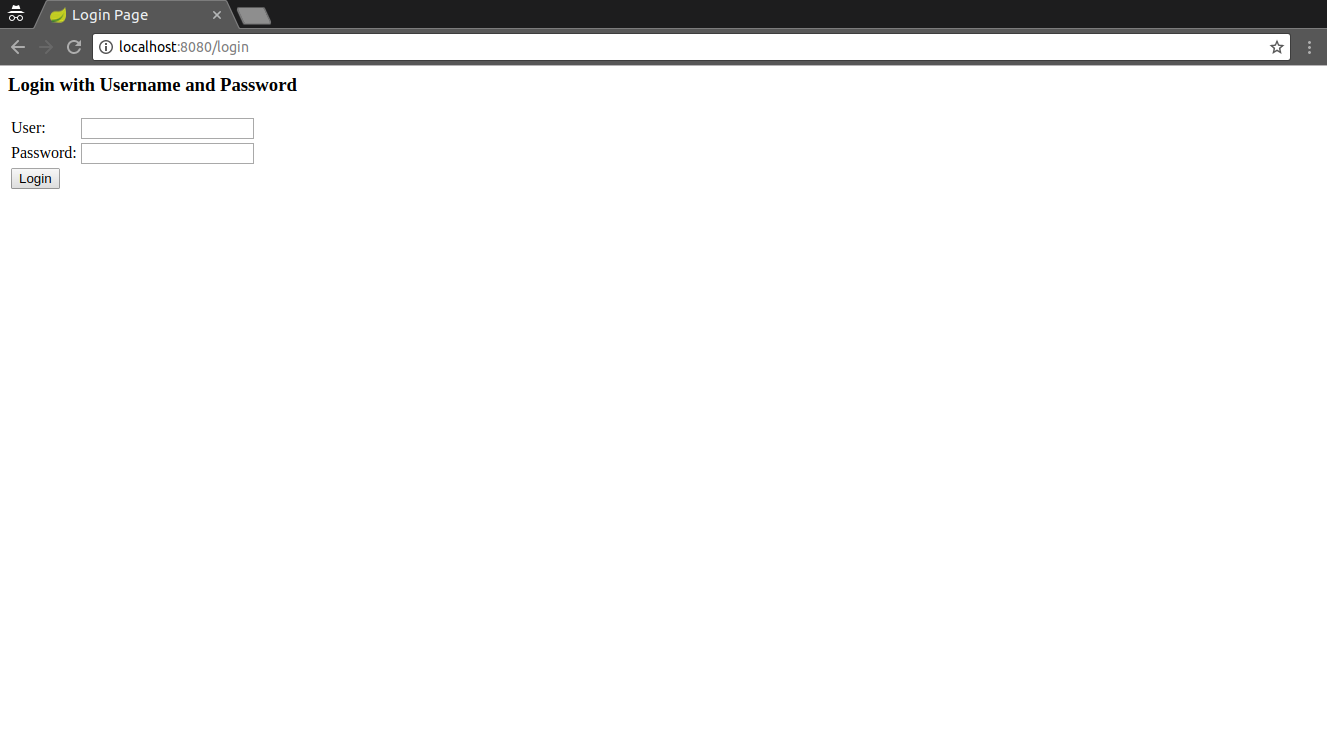
\includegraphics[width=1\textwidth]{./resources/020-custom-login}
		\caption{\textit{Username} dan \textit{Password Custom}}
		\label{ref:custom-login}
	\end{figure}
	
	Isikan dengan \textit{username} dan \textit{password} seperti pada kelas \texttt{SecurityConfig} pada baris ke-16 dan ke-17.	 Perhatikan pula bahwa pada halaman login ada kode \texttt{csrf} sebagai pengaman.
	
	\item Sampai sini, langkah konfigurasi \textit{security} untuk aplikasi \textit{web} yang kita bangun masih statis, \textit{username} dan \textit{password} masih harus \textit{hard-code}.

\end{enumerate}


\section{\textit{Username} dan \textit{Password} Dari DB}

Selanjutnya kita akan bangun sistem \textit{security} dengan \textit{username} dan \textit{password} yang dinamis yang datanya diambilkan dari sistem basis data.

Berikut adalah langkah-langkahnya :

\begin{enumerate}
	\item Buatlah struktur tabelnya terlebih dahulu, karena struktur tabel untuk Spring Security akan mengikuti pola aturan tertentu, berikut adalah beberapa tabel yang perlu dibuat :
	\begin{enumerate}[a.]
		\item Tabel \textit{User}. Nantinya dari tabel ini nama \textit{user} dan \textit{password} akan dicocokan. Struktur tabelnya dengan nama table \texttt{users} adalah sebagai berikut :
		
\begin{tabular}{| c | c | c |}
\hline
Kolom & Tipe & Keterangan \\
\hline
\hline
username & varchar(30) & not null primary key \\
\hline
password & varchar(200) & not null \\
\hline
enabled & boolean & \\
\hline
\end{tabular}		
		
		\item Tabel \textit{Role}. Nantinya daftar akses akan ditempatkan dalam tabel ini. Struktur tabelnya dengan nama tabel \texttt{roles} adalah sebagai berikut :
		
\begin{tabular}{| c | c | c |}
\hline
Kolom & Tipe & Keterangan \\
\hline
\hline
id & varchar(36) & not null primary key \\
\hline
role & varchar(200) & not null \\
\hline
\end{tabular}
		
		\item Tabel \textit{User-Role}. Nantinya masing-masing \textit{user} akan memiliki kewenangan tertentu berdasarkan \textit{role} yang diberikan atau dipasangkan pada tabel ini. Struktur tabelnya dengan nama tabel \texttt{user\_role} adalah sebagai berikut :
		
\begin{tabular}{| c | c | c |}
\hline
Kolom & Tipe & Keterangan \\
\hline
\hline
username & varchar(30) & not null \\
\hline
id\_role & varchar(36) & not null \\
\hline
\end{tabular}		
	\end{enumerate}
	
	\item Selanjutnya kita buat halaman login dengan tambahan Bootstrap untuk mempercantiknya. Lokasi dari \textit{file} \texttt{login.html} disimpan di dalam \textit{folder} \texttt{templates} seperti terlihat pada gambar \ref{fig:lokasi-login} berikut ini :
	
	\begin{figure}[H]
		\centering
		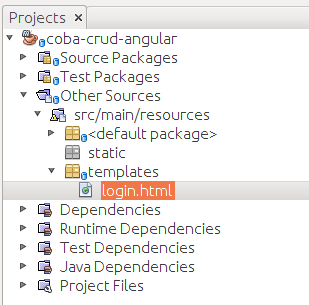
\includegraphics[width=0.5\textwidth]{./resources/022-lokasi-login}
		\caption{Lokasi \textit{file} \texttt{login.html}}
		\label{fig:lokasi-login}
	\end{figure}
	
	Isi dari \textit{file} \texttt{login.html} ini adalah sebagai berikut :
	
	\begin{lstlisting}
<html>
    <head>
        <title>Login</title>

        <link rel="stylesheet" href="https://maxcdn.bootstrapcdn.com/bootstrap/4.0.0-beta.2/css/bootstrap.min.css" integrity="sha384-PsH8R72JQ3SOdhVi3uxftmaW6Vc51MKb0q5P2rRUpPvrszuE4W1povHYgTpBfshb" crossorigin="anonymous">
        <script src="https://code.jquery.com/jquery-3.2.1.slim.min.js" integrity="sha384-KJ3o2DKtIkvYIK3UENzmM7KCkRr/rE9/Qpg6aAZGJwFDMVNA/GpGFF93hXpG5KkN" crossorigin="anonymous"></script>
		<script src="https://cdnjs.cloudflare.com/ajax/libs/popper.js/1.12.3/umd/popper.min.js" integrity="sha384-vFJXuSJphROIrBnz7yo7oB41mKfc8JzQZiCq4NCceLEaO4IHwicKwpJf9c9IpFgh" crossorigin="anonymous"></script>
		<script src="https://maxcdn.bootstrapcdn.com/bootstrap/4.0.0-beta.2/js/bootstrap.min.js" integrity="sha384-alpBpkh1PFOepccYVYDB4do5UnbKysX5WZXm3XxPqe5iKTfUKjNkCk9SaVuEZflJ" crossorigin="anonymous"></script>
    </head>

    <body>
        <div class="container">
        	<h1 div="card-title">Login</h1>
        	<form id="post" method="post" th:action="@{/login}">
        		<div class="card">
           			<div class="card-body">
               			<div class="container">
                   			<div class="row">
                       			<div class="col"><input name="username" type="text" class="form-control" placeholder="Username"/></div>
                   			</div>
                   			<div class="row">
                       			<div class="col"><input name="password" type="password" class="form-control" placeholder="Password"/></div>
                   			</div>
                   			<div class="row">
                       			<div class="col">
                           			<input type="submit" class="btn btn-primary" value="Masuk" />
                       			</div>
                   			</div>
               			</div>
           			</div>
       			</div>
       		</form>
    	</div>
    </body>
</html>
	\end{lstlisting}
	
	\item Mengubah kelas \texttt{SecurityConfig} agar melakukan \textit{override} terhadap \textit{method} \texttt{configureGlobal} dan menambahkan \textit{method} \texttt{configure(HttpSecurity)}. Berikut adalah perubahan kode dari kelas \texttt{SecurityConfig} :
	
	\begin{lstlisting}
package lab.aikibo.cobacrudangular.config;

import org.springframework.context.annotation.Configuration;
import org.springframework.security.config.annotation.web.configuration.WebSecurityConfigurerAdapter;
import org.springframework.security.config.annotation.web.servlet.configuration.EnableWebMvcSecurity;
import org.springframework.beans.factory.annotation.Autowired; 
import org.springframework.security.config.annotation.web.builders.HttpSecurity;
import org.springframework.security.config.annotation.authentication.builders.AuthenticationManagerBuilder;
import javax.sql.DataSource;
import org.springframework.security.web.csrf.CsrfTokenRepository;
import org.springframework.security.web.csrf.HttpSessionCsrfTokenRepository;
import lab.aikibo.cobacrudangular.util.CsrfHeaderFilter;
import org.springframework.security.config.annotation.web.builders.HttpSecurity;
import org.springframework.security.web.csrf.CsrfFilter;

@Configuration
@EnableWebMvcSecurity
public class SecurityConfig extends WebSecurityConfigurerAdapter {

	(*\textbf{\texttt{private static final String SQL\_LOGIN =  }}*)
	  (*\textbf{\texttt{"select username, password, enabled from users " + }}*)
	  (*\textbf{\texttt{"where username = ?"; }}*)

	(*\textbf{\texttt{private static final String SQL\_PERMISSION = }}*)
	  (*\textbf{\texttt{"select u.username, r.role as authority " + }}*)
	  (*\textbf{\texttt{"from users u " + }}*)
	  (*\textbf{\texttt{"join user\_role ur on u.username = ur.username " + }}*)
	  (*\textbf{\texttt{"join roles r on r.id = ur.id\_role " + }}*)
	  (*\textbf{\texttt{"where u.username = ?"; }}*)

	(*\textbf{\texttt{@Autowired }}*)
	(*\textbf{\texttt{private DataSource ds; }}*)
	
	@Autowired
	public void configureGlobal(AuthenticationManagerBuilder auth) throws Exception {
	  (*\textbf{\texttt{auth.jdbcAuthentication() }}*)
	    (*\textbf{\texttt{.dataSource(ds) }}*)
	    (*\textbf{\texttt{.usersByUsernameQuery(SQL\_LOGIN) }}*)
	    (*\textbf{\texttt{.authoritiesByUsernameQuery(SQL\_PERMISSION); }}*)
	}

	(*\textbf{\texttt{@Override }}*)
	(*\textbf{\texttt{protected void configure(HttpSecurity http) throws Exception \{ }}*)
	  (*\textbf{\texttt{http }}*)
	    (*\textbf{\texttt{.authorizeRequests() }}*)
	      (*\textbf{\texttt{.anyRequest().authenticated() }}*)
	    (*\textbf{\texttt{.and() }}*)
	      (*\textbf{\texttt{.formLogin().loginPage("/login").permitAll() }}*)
	      (*\textbf{\texttt{.defaultSuccessUrl("/") }}*)
	    (*\textbf{\texttt{.and() }}*)
	      (*\textbf{\texttt{.logout() }}*)
	    (*\textbf{\texttt{.and() }}*)
	      (*\textbf{\texttt{.addFilterAfter(new CsrfHeaderFilter(), }}*)
	        (*\textbf{\texttt{CsrfFilter.class) }}*)
	      (*\textbf{\texttt{.csrf() }}*)
	        (*\textbf{\texttt{.csrfTokenRepository(csrfTokenRepository()); }}*)
	(*\textbf{\texttt{\} }}*)

	(*\textbf{\texttt{private CsrfTokenRepository csrfTokenRepository() \{ }}*)
	  (*\textbf{\texttt{HttpSessionCsrfTokenRepository tokenRepo = }}*)
	    (*\textbf{\texttt{new HttpSessionCsrfTokenRepository(); }}*)
	  (*\textbf{\texttt{tokenRepo.setHeaderName("X-XSRF-TOKEN"); }}*)
	  (*\textbf{\texttt{return tokenRepo; }}*)
	(*\textbf{\texttt{\} }}*)

}
	\end{lstlisting}
	
	Pada baris ke-36, kita sudah mulai melakukan otentikasi \textit{username} dan \textit{password} dari sistem basis data. 
	
	Pada baris ke-43 adalah tempat kita mengatur halaman mana yang boleh dibuka oleh umum, dan mana yang hanya boleh setelah \textit{login} bahkan pada \textit{method} ini pun dapat diberikan akses lebih spesifik terhadap \textit{user} mana yang boleh melakukan akses ke \textit{url} tertentu.
	
	Pada baris ke-56 adalah cara atau mekanisme yang dilakukan Spring untuk menyampaikan CSRF dari \textit{user} yang melakukan akses, dimana implementasinya dilakukan pada \textit{method} di baris ke-59, yaitu dengan cara menyematkan atau menempelkan informasi CSRF di \textit{header} tiap \textit{request}.
	
	\item Karena kita membuat halaman \textit{login} khusus yang kita desain sendiri, maka halaman ini harus didaftarkan terlebih dahulu, mirip seperti saat kita buat aplikasi dengan \texttt{Thymeleaf} sebelumnya yang memerlukan \textit{mapping}, namun kali ini dengan cara yang berbeda. Kali ini kita akan membuat sebuah kelas dengan nama \texttt{WebConfig} yang menjadi tempat untuk mendaftarkan setiap \textit{View} yang kita buat. Letak \textit{file} dari \texttt{WebConfig} ini adalah seperti pada gambar \ref{fig:letak-WebConfig} berikut :
	
	\begin{figure}[H]
		\centering
		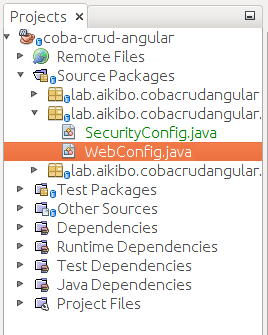
\includegraphics[width=0.5\textwidth]{./resources/023-lokasi-webconfig}
		\caption{Lokasi \textit{File} \texttt{WebConfig}}
		\label{fig:letak-WebConfig}
	\end{figure}
	
	Isi kode dari \textit{file} ini adalah sebagai berikut :
	
	\begin{lstlisting}
package lab.aikibo.cobacrudangular.config;

import org.springframework.context.annotation.Configuration;
import org.springframework.web.servlet.config.annotation.ViewControllerRegistry;
import org.springframework.web.servlet.config.annotation.WebMvcConfigurerAdapter;

@Configuration
public class WebConfig extends WebMvcConfigurerAdapter {

	@Override
	public void addViewControllers(ViewControllerRegistry registry) {
		registry.addViewController("/login").setViewName("login");
	}

}
	\end{lstlisting}
	
	\item Lalu melakukan pemeriksaan aplikasi, seharusnya aplikasi akan menampilkan halaman \textit{login} yang telah kita bangun sendiri seperti pada gambar \ref{fig:halaman-login} berikut :
	
	\begin{figure}[H]
		\centering
		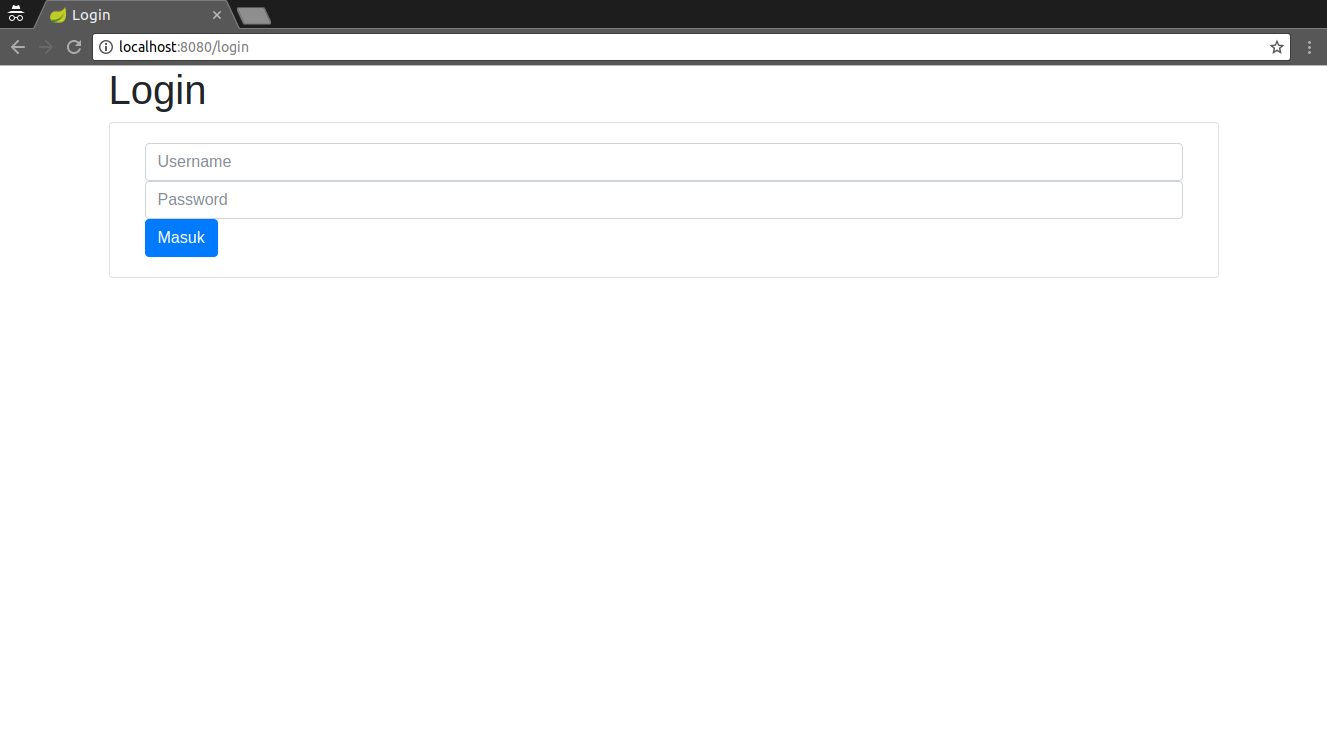
\includegraphics[width=1\textwidth]{./resources/024-halaman-login}
		\caption{Halaman \textit{Login} Yang Dibangun Sendiri}
		\label{fig:halaman-login}
	\end{figure}
	
	Dan apabila berhasil \textit{login} maka akan muncul halaman seperti pada gambar \ref{fig:halaman-utama} berikut :
	
	\begin{figure}[H]
		\centering
		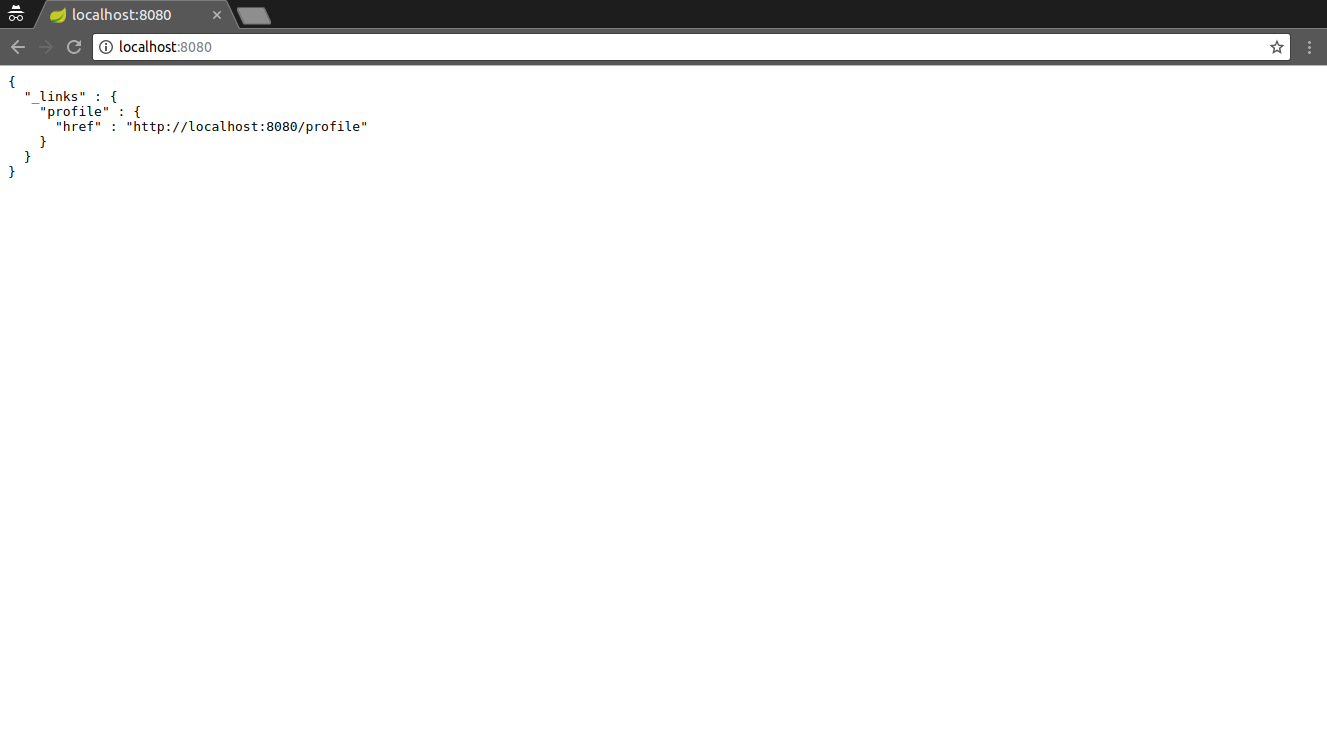
\includegraphics[width=1\textwidth]{./resources/025-halaman-utama}
		\caption{Halaman Setelah \textit{Login} Berhasil}
		\label{fig:halaman-utama}
	\end{figure}	
	
\end{enumerate}


\section{Mencoba Angular}

Karena kita sudah berhasil membuat bagian \textit{login} berjalan dengan semestinya, kali ini kita akan mencoba mengawali pembahasan Angular dengan cara sederhana. Kita akan membuat sebuah halaman interaktif yang dapat langsung berubah ketika \textit{user} melakukan aksi di sebuah halaman. Berikut adalah langkahnya :

\begin{enumerate}
	\item Kita akan membuat sebuah halaman \texttt{html} terlebih dahulu, misalkan kita beri nama \texttt{test-angular.html}. Lokasi dari \textit{file} ini adalah seperti pada gambar \ref{fig:lokasi-test-angular} berikut :
	
	\begin{figure}[H]
		\centering
		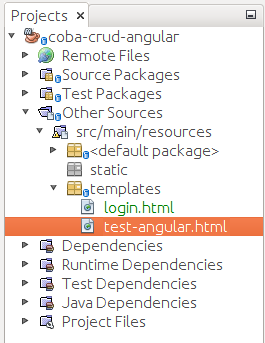
\includegraphics[width=0.5\textwidth]{./resources/026-lokasi-test-angular}
		\caption{Lokasi \textit{File} \texttt{test-angular.html}}
		\label{fig:lokasi-test-angular}
	\end{figure}
	
	Isi dari kode programnya adalah sebagai berikut :
	
	\begin{lstlisting}
<html>
<head>
	<title>Percobaan Angular</title>

    <link rel="stylesheet" href="https://maxcdn.bootstrapcdn.com/bootstrap/4.0.0-beta.2/css/bootstrap.min.css" integrity="sha384-PsH8R72JQ3SOdhVi3uxftmaW6Vc51MKb0q5P2rRUpPvrszuE4W1povHYgTpBfshb" crossorigin="anonymous"/>
    <script src="https://code.jquery.com/jquery-3.2.1.slim.min.js" integrity="sha384-KJ3o2DKtIkvYIK3UENzmM7KCkRr/rE9/Qpg6aAZGJwFDMVNA/GpGFF93hXpG5KkN" crossorigin="anonymous"></script>
    <script src="https://cdnjs.cloudflare.com/ajax/libs/popper.js/1.12.3/umd/popper.min.js" integrity="sha384-vFJXuSJphROIrBnz7yo7oB41mKfc8JzQZiCq4NCceLEaO4IHwicKwpJf9c9IpFgh" crossorigin="anonymous"></script>
    <script src="https://maxcdn.bootstrapcdn.com/bootstrap/4.0.0-beta.2/js/bootstrap.min.js" integrity="sha384-alpBpkh1PFOepccYVYDB4do5UnbKysX5WZXm3XxPqe5iKTfUKjNkCk9SaVuEZflJ" crossorigin="anonymous"></script>
    <script src="https://ajax.googleapis.com/ajax/libs/angularjs/1.6.6/angular.min.js"></script>
</head>
<body ng-app="">
	Isikan nama <input type="text" ng-model="nama" />
	<br />
	Selamat datang, {{ nama }}
</body>
</html>
	\end{lstlisting}
	
	Yang perlu diperhatikan adalah pada baris ke-9, kita menambahkan \textit{script} untuk AngularJS, agar AngularJS dapat kita gunakan. Kemudian pada baris ke-12, ada parameter \texttt{ng-model} yang isinya adalah pembentukan sebuah variabel pada AngularJS dengan nama \texttt{nama}. Nantinya variabel ini akan dipanggil / dibaca pda baris ke-14.
	
	\item Registrasikan halaman ini di \texttt{WebConfig}, sehingga kelas \texttt{WebConfig} menjadi seperti ini :
	
	\begin{lstlisting}
package lab.aikibo.cobacrudangular.config;

import org.springframework.context.annotation.Configuration;
import org.springframework.web.servlet.config.annotation.ViewControllerRegistry;
import org.springframework.web.servlet.config.annotation.WebMvcConfigurerAdapter;

@Configuration
public class WebConfig extends WebMvcConfigurerAdapter {

	@Override
	public void addViewControllers(ViewControllerRegistry registry) {
		registry.addViewController("/login").setViewName("login");
	    (*\textbf{\texttt{registry.addViewController("/test-angular") }}*)
	      (*\textbf{\texttt{.setViewName("test-angular"); }}*)
	}

}
	\end{lstlisting}
	
	Sehingga apabila ada \textit{request} ke \textit{url} \texttt{/test-angular}	 akan di \textit{respon} dengan halaman \texttt{test-angular.html}.
	
	\item Melakukan uji coba aplikasi, seharusnya apabila alamat \textit{url} diarahkan ke \texttt{localhost:8080/test-angular}, nantinya akan aplikasi akan meminta informasi \textit{login}, dan setelah berhasil \textit{login}, nanti akan dibawa ke halaman seperti pada gambar \ref{fig:halaman-test-angular} berikut :
	
	\begin{figure}[H]
		\centering
		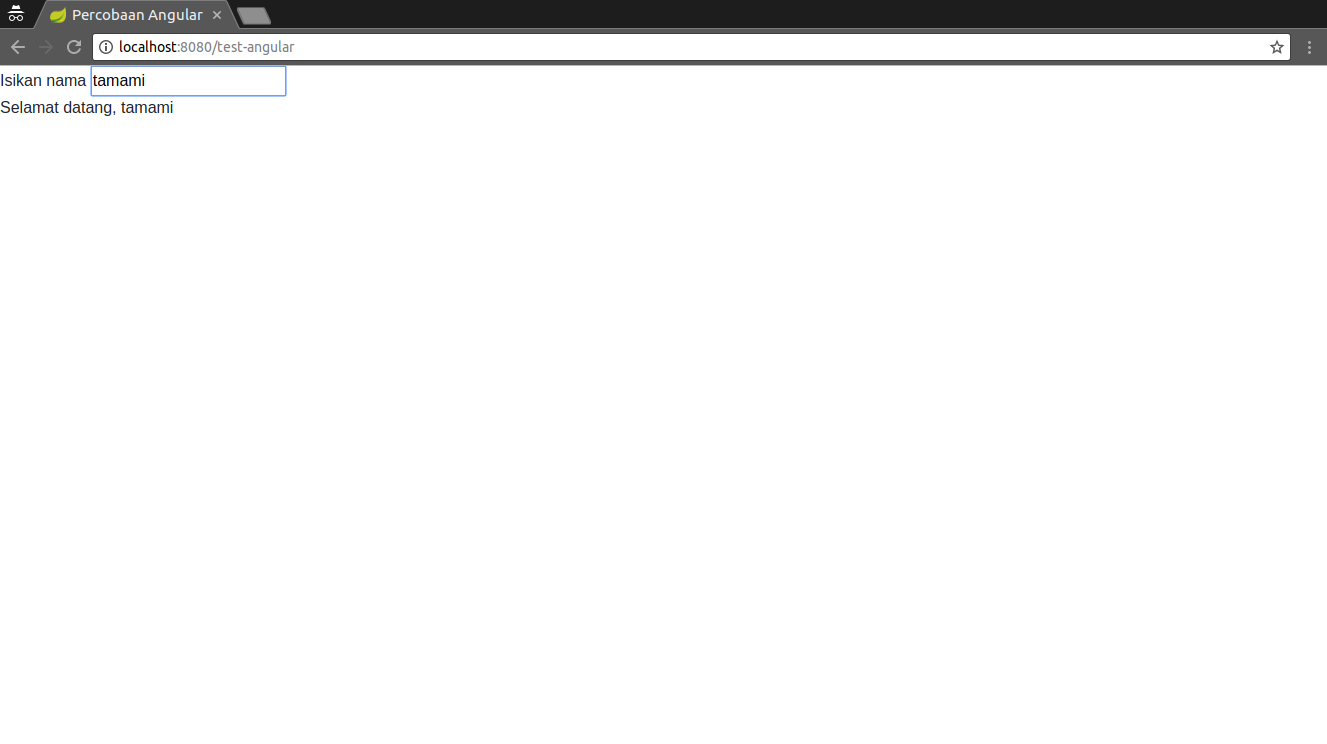
\includegraphics[width=1\textwidth]{./resources/027-test-angular}
		\caption{Halaman \texttt{test-angular.html}}
		\label{fig:halaman-test-angular}
	\end{figure}
	
	Bila \textit{user} mengisikan nama ditempat yang disediakan, aplikasi dapat langsung melakukan respon interaktif tanpa harus melakukan \textit{request} ke \textit{server}.	
	
\end{enumerate}


\section{Tampilkan Data}

Sekarang kita coba tampilkan isi dari basis data ke halaman \textit{web} kita dengan Angular, berikut langkah-langkahnya :

\begin{enumerate}
	\item Yang pertama kita lakukan adalah membuat tampilan \textit{front-end} terlebih dahulu, yaitu daftar mahasiswa dalam sebuah tabel, kita sebut saja nama \textit{file} untuk ini adalah \texttt{daftar-mahasiswa.html}, lokasi \textit{file} dapat dilihat seperti pada gambar \ref{fig:lokasi-daftar-mahasiswa} berikut :
	
	\begin{figure}[H]
		\centering
		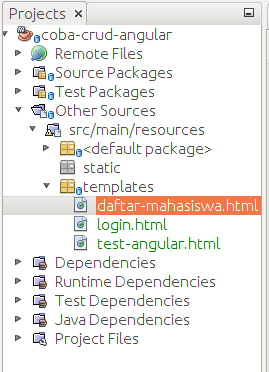
\includegraphics[width=0.5\textwidth]{./resources/028-lokasi-daftar-mahasiswa}
		\caption{Lokasi \textit{File} \texttt{daftar-mahasiswa.html}}
		\label{fig:lokasi-daftar-mahasiswa}
	\end{figure}
	
	Isi dari \textit{file} \texttt{daftar-mahasiswa.html} ini adalah sebagai berikut :
	
	\begin{lstlisting}
<html>
<head>
        <title>Aplikasi Pendataan Mahasiswa</title>
    <link rel="stylesheet" href="https://maxcdn.bootstrapcdn.com/bootstrap/4.0.0-beta.2/css/bootstrap.min.css" integrity="sha384-PsH8R72JQ3SOdhVi3uxftmaW6Vc51MKb0q5P2rRUpPvrszuE4W1povHYgTpBfshb" crossorigin="anonymous"/>
    <script src="https://code.jquery.com/jquery-3.2.1.slim.min.js" integrity="sha384-KJ3o2DKtIkvYIK3UENzmM7KCkRr/rE9/Qpg6aAZGJwFDMVNA/GpGFF93hXpG5KkN" crossorigin="anonymous"></script>
    <script src="https://cdnjs.cloudflare.com/ajax/libs/popper.js/1.12.3/umd/popper.min.js" integrity="sha384-vFJXuSJphROIrBnz7yo7oB41mKfc8JzQZiCq4NCceLEaO4IHwicKwpJf9c9IpFgh" crossorigin="anonymous"></script>
    <script src="https://maxcdn.bootstrapcdn.com/bootstrap/4.0.0-beta.2/js/bootstrap.min.js" integrity="sha384-alpBpkh1PFOepccYVYDB4do5UnbKysX5WZXm3XxPqe5iKTfUKjNkCk9SaVuEZflJ" crossorigin="anonymous"></script>
    <script src="https://ajax.googleapis.com/ajax/libs/angularjs/1.6.6/angular.min.js"></script>
    <script src="/js/app.js"></script>
    <script src="/js/api-controller.js"></script>
</head>
<body ng-app="MahasiswaApp" class="container" >

    <div class="jumbotron">
        <h1>Daftar Mahasiswa</h1>
    </div>

    <div ng-controller="ApiController">

        <table class="table table-striped">
            <thead>
                <tr>
                    <th scope="col">NIM</th>
                    <th scope="col">NAMA</th>
                    <th scope="col">JURUSAN</th>
                </tr>
            </thead>
            <tbody>
                <tr ng-repeat="mhs in daftarMahasiswa">
                    <td>{{mhs.nim}}</td>
                    <td>{{mhs.nama}}</td>
                    <td>{{mhs.jurusan}}</td>
                </tr>
            </tbody>            
        </table>
    </div>
</body>
</html>
	\end{lstlisting}	
	
	Kita coba beda satu per satu, dari baris ke-12, ada deklarasi \texttt{ng-app} dengan nilai \texttt{MahasiswaApp} yang sebetulnya diambilkan dari \textit{app.js}, letak \textit{file} dari \texttt{app.js} ini seperti ditunjukkan pada gambar \ref{fig:lokasi-app-js} berikut :
	
	\begin{figure}[H]
		\centering
		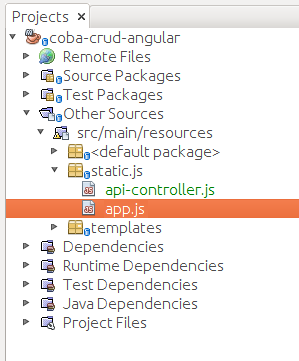
\includegraphics[width=0.5\textwidth]{./resources/029-lokasi-app-js}
		\caption{Lokasi \textit{File} \texttt{app.js}}
		\label{fig:lokasi-app-js}
	\end{figure}
	
	Sedangkan isi dari \textit{file} \texttt{app.js} ini adalah sebagai berikut :
	
	\begin{lstlisting}
var app = angular.module('MahasiswaApp', []);
	\end{lstlisting}
	
	Lalu pada baris ke-18 ada deklarasi \texttt{ng-controller} dengan nilai / isian \texttt{ApiController} yang sebetulnya diambilkan dari \textit{file} \texttt{api-controller.js}. Lokasi \textit{file} \texttt{api-controller.js} ini seperti ditunjukkan pada gambar \ref{fig:lokasi-api-controller-js} berikut :
	
	\begin{figure}[H]
		\centering
		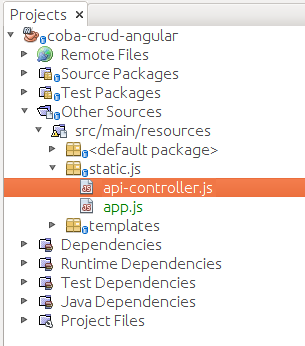
\includegraphics[width=0.5\textwidth]{./resources/030-lokasi-api-controller-js}
		\caption{Lokasi \textit{File} \texttt{api-controller.js}}
		\label{fig:lokasi-api-controller-js}
	\end{figure}
	
	Isi dari \textit{file} ini adalah sebagai berikut :
	
	\begin{lstlisting}
app.controller('ApiController', function($scope, $http) {
    $scope.daftarMahasiswa = {};
    
    $scope.updateDaftarMahasiswa = function() {
      $http.get('daftar-mahasiswa').then(sukses, gagal);
      
      function sukses(response) {
          console.log(response);
          $scope.daftarMahasiswa = response.data;
      };
      
      function gagal(response) {
          console.log(response);
      }
    };
    
    $scope.updateDaftarMahasiswa();
});
	\end{lstlisting}
	
	Di \textit{file} \texttt{api-controller} inilah nantinya \textit{front-end} akan berkomunikasi dengan \textit{back-end}. Pada \texttt{ApiController} milik Angular ini, pada baris ke-2 akan menyiapkan sebuah variabel \texttt{daftarMahasiswa} yang masih kosong.
	
	Kemudian pada baris ke-4 ada deklarasi fungsi dengan nama \texttt{updateDaftarMahasiswa}, dimana didalamnya melakukan \textit{request} ke \textit{server} dengan \textit{method} \texttt{get} ke alamat \texttt{/daftar-mahasiswa}, yang diharapkan, pada saat sukses melakukan \textit{request} dan menerima \textit{response} yang benar, sehingga variabel \texttt{daftarMahasiswa} dapat diisikan dengan data dari \textit{server} seperti pada baris ke-9.
	
	Setiap dilakukan \textit{refresh} / \textit{reload} halaman, maka akan dipanggil fungsi \texttt{updateDaftarMahasiswa} seperti pada baris ke-17.
	
	Kita kembali lagi ke \textit{file} \texttt{daftar-mahasiswa.html} pada baris ke-29, dimana disana ada atribut \texttt{ng-repeat} dengan isian \texttt{mhs in daftarMahasiswa}, nantinya Angular akan melakukan iterasi untuk setiap data pada \texttt{daftarMahasiswa} disimpan dalam variabel temporer \texttt{mhs}, yang kemudian ditampilkan di tiap baris seperti disebutkan pada baris ke-30, 31, dan 32.
	
	Sampai sini \textit{back-end} diharapkan dapat menyiapkan \textit{mapping} ke \textit{url} \texttt{/daftar-mahasiswa} dengan nilai kembalian yang didalamnya terdapat data larik dari daftar mahasiswa, untuk selanjutnya disimpan dalam variabel \texttt{daftarMahasiswa}.
	
	\item Menyiapkan \textit{controller} agar dapat melakukan \textit{response} terhadap \textit{url} \texttt{/daftar-mahasiswa}, \textit{file controller} yang kita buat misalkan dengan nama \texttt{ApiRestController} dengan letak \textit{file} berada seperti ditunjukkan pada gambar \ref{fig:letak-api-rest-controller} berikut :
	
	\begin{figure}[H]
		\centering
		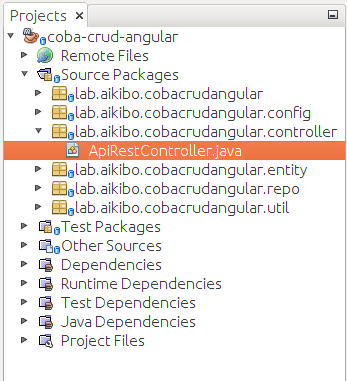
\includegraphics[width=0.5\textwidth]{./resources/031-letak-api-rest-controller}
		\caption{Letak \textit{File} \texttt{ApiRestController.java}}
		\label{fig:letak-api-rest-controller}
	\end{figure}
	
	Isi dari kelas \texttt{ApiRestController} ini adalah sebagai berikut :
	
	\begin{lstlisting}
package lab.aikibo.cobacrudangular.controller;

import java.util.List;
import lab.aikibo.cobacrudangular.entity.Mahasiswa;
import lab.aikibo.cobacrudangular.repo.MahasiswaRepo;
import org.springframework.beans.factory.annotation.Autowired;
import org.springframework.web.bind.annotation.RequestMapping;
import org.springframework.web.bind.annotation.RestController;

/**
 *
 * @author tamami <tamami.oka@gmail.com>
 */
@RestController
public class ApiRestController {
    
    @Autowired
    private MahasiswaRepo mhsRepo;
    
    @RequestMapping("/daftar-mahasiswa")
    public List<Mahasiswa> getDaftarMahasiswa() {
        return mhsRepo.findAll();
    }
    
}
	\end{lstlisting}
	
	Hanya ada sebuah \textit{method} dengan nama \texttt{getDaftarMahasiswa} dengan \textit{mapping} ke \textit{url} \texttt{/daftar-mahasiswa}. Isi dari \textit{method} ini pun sangat sederhana, hanya memanggil \textit{method} \texttt{findAll} dari \texttt{MahasiswaRepo}, objek inilah yang nantinya akan memberikan kita akses operasi terhadap basis data.
	
	\item Membuat kelas \texttt{Mahasiswa} yang digunakan sebagai \textit{mapping} kelas dari tabel di basis data, letak \textit{file} \texttt{Mahasiswa.java} ini seperti ditunjukkan pada gambar \ref{fig:letak-mahasiswa} berikut :
	
	\begin{figure}[H]
		\centering
		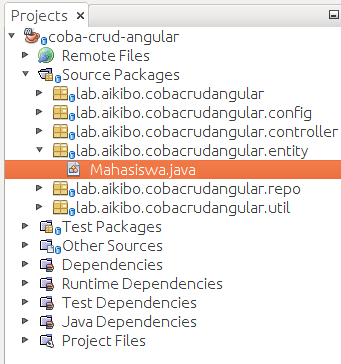
\includegraphics[width=0.5\textwidth]{./resources/032-letak-mahasiswa}
		\caption{Letak \textit{File} \texttt{Mahasiswa.java}}
		\label{fig:letak-mahasiswa}
	\end{figure}
	
	Isi dari \textit{file} \texttt{Mahasiswa.java} ini adalah sebagai berikut :
	
	\begin{lstlisting}
package lab.aikibo.cobacrudangular.entity;

import javax.persistence.Column;
import javax.persistence.Entity;
import javax.persistence.Id;
import lombok.Getter;
import lombok.Setter;

/**
 *
 * @author tamami <tamami.oka@gmail.com>
 */
@Entity
public class Mahasiswa {
    
    @Id @Getter @Setter
    private String nim;
    
    @Column @Getter @Setter
    private String nama;
    
    @Column @Getter @Setter
    private String jurusan;
    
}
	\end{lstlisting}
	
	Kelas ini ditandai dengan anotasi \texttt{@Entity}, dan di dalamnya berisi atribut yang sesuai dengan nama kolom yang ada pada tabel di sistem basis data, dimana anotasi \texttt{@Id} menandakan \textit{primary key} di sistem basis data, dan anotasi \texttt{@Column} tentunya menandakan atribut kolom di sistem basis data.
	
	Kita juga memanfaatkan anotasi \texttt{@Getter} dan \texttt{@Setter} milik Lombok agar kode yang kita bangun lebih bersih dan mudah dibaca.
	
	\item Selanjutnya kita membuat \textit{file} dengan nama \texttt{MahasiswaRepo.java} yang nantinya ditugaskan untuk membuat \textit{query} operasi terhadap sistem basis data. Letak \textit{file} \texttt{MahasiswaRepo.java} ini seperti ditunjukkan pada gambar \ref{fig:letak-mahasiswa-repo} berikut :
	
	\begin{figure}[H]
		\centering
		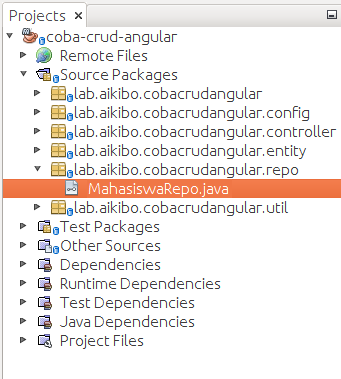
\includegraphics[width=0.5\textwidth]{./resources/033-letak-mahasiswa-repo}
		\caption{Letak \textit{File} \texttt{MahasiswaRepo.java}}
		\label{fig:letak-mahasiswa-repo}
	\end{figure}
	
	Isi dari \textit{file} ini juga cukup sederhana, berikut kodenya :
	
	\begin{lstlisting}
package lab.aikibo.cobacrudangular.repo;

import lab.aikibo.cobacrudangular.entity.Mahasiswa;
import org.springframework.data.jpa.repository.JpaRepository;
import org.springframework.stereotype.Repository;

/**
 *
 * @author tamami <tamami.oka@gmail.com>
 */
@Repository
public interface MahasiswaRepo extends JpaRepository<Mahasiswa, String> {
   
}
	\end{lstlisting}
	
	\textit{Interface} ini ditandai dengan anotasi \texttt{@Repository} agar kita dapat melakukan \textit{dependency injection} terhadap objek ini, yang implementasinya dapat dilihat di \textit{file} \texttt{ApiRestController.java} pada baris ke-18, yaitu pada deklarasi objek \texttt{mhsRepo} dengan anotasi \texttt{@Autowired}. 
	
	\item Langkah berikutnya yang perlu dikerjakan adalah mendaftarkan halaman \texttt{daftar-mahasiswa.html} ke dalam daftar \textit{view} pada kelas \texttt{WebConfig} dengan isi kode sebagai berikut :
	
	\begin{lstlisting}
package lab.aikibo.cobacrudangular.config;

import org.springframework.context.annotation.Configuration;
import org.springframework.web.servlet.config.annotation.ViewControllerRegistry;
import org.springframework.web.servlet.config.annotation.WebMvcConfigurerAdapter;

@Configuration
public class WebConfig extends WebMvcConfigurerAdapter {

	@Override
	public void addViewControllers(ViewControllerRegistry registry) {
		registry.addViewController("/login").setViewName("login");
		registry.addViewController("/test-angular").setViewName("test-angular");
        (*\textbf{\texttt{registry.addViewController("/") }}*)       
            (*\textbf{\texttt{.setViewName("daftar-mahasiswa"); }}*)
        (*\textbf{\texttt{registry.addViewController("/daftar-mahasiswa") }}*)
            (*\textbf{\texttt{.setViewName("daftar-mahasiswa"); }}*)
	}
}
	\end{lstlisting}
	
	\item Langkah terakhir adalah melakukan uji coba terhadap aplikasi yang kita bangun, setelah aplikasi dijalankan nantinya seperti biasa akan menampilkan halaman \textit{login}, setelah berhasil, maka seharusnya halaman yang tampil adalah seperti pada gambar \ref{fig:halaman-daftar-mahasiswa} berikut ini :
	
	\begin{figure}[H]
		\centering
		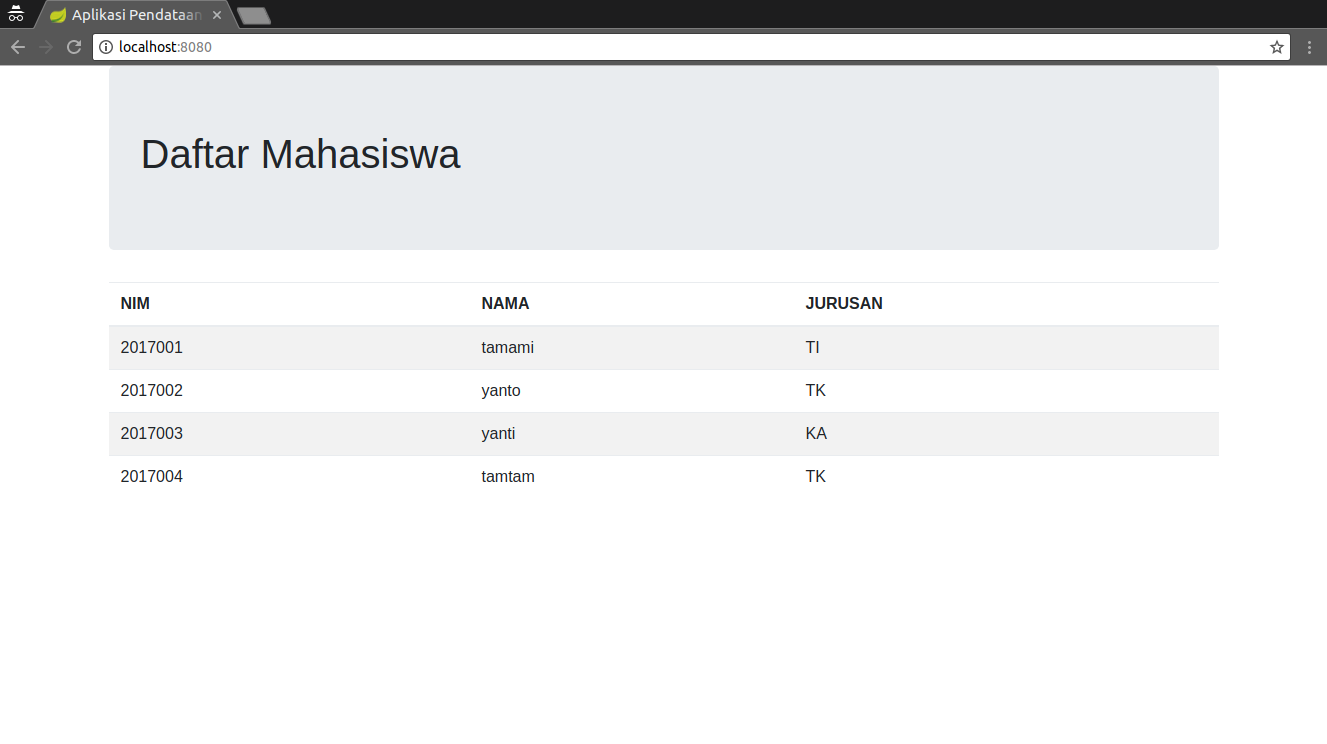
\includegraphics[width=1\textwidth]{./resources/034-halaman-daftar-mahasiswa}
		\caption{Halaman Daftar Mahasiswa}
		\label{fig:halaman-daftar-mahasiswa}
	\end{figure}
\end{enumerate}

Sampai sini aplikasi \textit{web} kita telah dilengkapi dengan fasilitas untuk menampilkan daftar Mahasiswa.


\section{Tambah Data}

Untuk menambahkan data, kita perlu sebuah halaman yang berbentuk seperti formulir agar \textit{user} dapat mengisikan informasi tentang data yang baru. Langkah-langkahnya adalah sebagai berikut :

\begin{enumerate}

	\item Pertama kita berikan tombol di bawah daftar mahasiswa untuk membuka halaman formulir isian data mahasiswa baru, berikut perubahan yang kita lakukan di \textit{file} \texttt{daftar-mahasiswa.html} :

\begin{lstlisting}
<html>
<head>
        <title>Aplikasi Pendataan Mahasiswa</title>
    <link rel="stylesheet" href="https://maxcdn.bootstrapcdn.com/bootstrap/4.0.0-beta.2/css/bootstrap.min.css" integrity="sha384-PsH8R72JQ3SOdhVi3uxftmaW6Vc51MKb0q5P2rRUpPvrszuE4W1povHYgTpBfshb" crossorigin="anonymous"/>
    <script src="https://code.jquery.com/jquery-3.2.1.slim.min.js" integrity="sha384-KJ3o2DKtIkvYIK3UENzmM7KCkRr/rE9/Qpg6aAZGJwFDMVNA/GpGFF93hXpG5KkN" crossorigin="anonymous"></script>
    <script src="https://cdnjs.cloudflare.com/ajax/libs/popper.js/1.12.3/umd/popper.min.js" integrity="sha384-vFJXuSJphROIrBnz7yo7oB41mKfc8JzQZiCq4NCceLEaO4IHwicKwpJf9c9IpFgh" crossorigin="anonymous"></script>
    <script src="https://maxcdn.bootstrapcdn.com/bootstrap/4.0.0-beta.2/js/bootstrap.min.js" integrity="sha384-alpBpkh1PFOepccYVYDB4do5UnbKysX5WZXm3XxPqe5iKTfUKjNkCk9SaVuEZflJ" crossorigin="anonymous"></script>
    <script src="https://ajax.googleapis.com/ajax/libs/angularjs/1.6.6/angular.min.js"></script>
    <script src="/js/app.js"></script>
    <script src="/js/api-controller.js"></script>
</head>
<body ng-app="MahasiswaApp" class="container" >

    <div class="jumbotron">
        <h1>Daftar Mahasiswa</h1>
    </div>

    <div ng-controller="ApiController">

        <table class="table table-striped">
            <thead>
                <tr>
                    <th scope="col">NIM</th>
                    <th scope="col">NAMA</th>
                    <th scope="col">JURUSAN</th>
                </tr>
            </thead>
            <tbody>
                <tr ng-repeat="mhs in daftarMahasiswa">
                    <td>{{mhs.nim}}</td>
                    <td>{{mhs.nama}}</td>
                    <td>{{mhs.jurusan}}</td>
                </tr>
            </tbody>            
            (*\textbf{\texttt{<tfoot> }}*)
              (*\textbf{\texttt{<tr> }}*)
                (*\textbf{\texttt{<td> }}*)
                  (*\textbf{\texttt{<a class="btn btn-primary" }}*)
                      (*\textbf{\texttt{href="/form" role="button"> }}*)
                    (*\textbf{\texttt{Tambah</a> }}*)
                (*\textbf{\texttt{</td> }}*)
              (*\textbf{\texttt{</tr> }}*)
            (*\textbf{\texttt{</tfoot> }}*)
        </table>
    </div>
</body>
</html>
\end{lstlisting}

	Perhatikan pada baris ke-38 dimana kita menambahkan element \texttt{a} yang melakukan \textit{request} ke \textit{server} dengan \textit{url} \texttt{/form} dan menggunakan Bootstrap untuk menjadikan \textit{link} ini seperti sebuah tombol.
	
	\item Hal berikutnya yang disiapkan adalah \textit{file} \texttt{form.html} sebagai bahan \textit{response} atas \textit{request} sebelumnya. Letak \textit{file} \texttt{form.html} ini sama seperti \textit{file} \texttt{html} lainnya yaitu di dalam \textit{folder} \texttt{templates}, isi kode dari \textit{file} \texttt{form.html} ini adalah sebagai berikut :
	
	\begin{lstlisting}
<html>
<head>
    <title>Form Entry Data</title>
    
    <link rel="stylesheet" href="https://maxcdn.bootstrapcdn.com/bootstrap/4.0.0-beta.2/css/bootstrap.min.css" integrity="sha384-PsH8R72JQ3SOdhVi3uxftmaW6Vc51MKb0q5P2rRUpPvrszuE4W1povHYgTpBfshb" crossorigin="anonymous"/>
    <script src="https://code.jquery.com/jquery-3.2.1.slim.min.js" integrity="sha384-KJ3o2DKtIkvYIK3UENzmM7KCkRr/rE9/Qpg6aAZGJwFDMVNA/GpGFF93hXpG5KkN" crossorigin="anonymous"></script>
    <script src="https://cdnjs.cloudflare.com/ajax/libs/popper.js/1.12.3/umd/popper.min.js" integrity="sha384-vFJXuSJphROIrBnz7yo7oB41mKfc8JzQZiCq4NCceLEaO4IHwicKwpJf9c9IpFgh" crossorigin="anonymous"></script>
    <script src="https://maxcdn.bootstrapcdn.com/bootstrap/4.0.0-beta.2/js/bootstrap.min.js" integrity="sha384-alpBpkh1PFOepccYVYDB4do5UnbKysX5WZXm3XxPqe5iKTfUKjNkCk9SaVuEZflJ" crossorigin="anonymous"></script>
    <script src="https://ajax.googleapis.com/ajax/libs/angularjs/1.6.6/angular.min.js"></script>
    <script src="/js/app.js"></script>
    <script src="/js/form-controller.js"></script>
</head>
<body ng-app="MahasiswaApp">
    <div class="container" ng-controller="FormController">
        <div class="jumbotron">
            <h1>Formulir Isian</h1>
        </div>
        
<form>
    <div class="form-group row">
        <label class="col-sm-2 col-form-label">NIM</label>
        <input class="form-control" type="text" placeholder="NIM" ng-model="dataMahasiswa.nim" />
    </div>
    <div class="form-group row">
        <label class="col-sm-2 col-form-label">Nama</label>
        <input class="form-control" type="text" placeholder="Nama" ng-model="dataMahasiswa.nama"/>
    </div>
    <div class="form-group row">
        <label class="col-sm-2 col-form-label">Jurusan</label>
        <input class="form-control" type="text" placeholder="Usia" ng-model="dataMahasiswa.jurusan" />
    </div>    
    <div class="form-group row">
        <button class="btn btn-primary" ng-click="simpan()">Simpan</button>
    </div>
</form>
    </div>
</body>
</html>
	\end{lstlisting}
	
	Seperti pada \textit{file} \texttt{daftar-mahasiswa.html}, disini kita juga menyertakan parameter \texttt{ng-app} dengan isi \texttt{MahasiswaApp} seperti pada baris ke-13 berikut :
	
	\begin{lstlisting}[firstnumber=13]
<body ng-app="MahasiswaApp"> \end{lstlisting}

	Kemudian pada baris ke-14 kita mengaitkan komponen \texttt{<div>} dengan \textit{controller} Angular \texttt{FormController} seperti berikut :
	
	\begin{lstlisting}[firstnumber=14]
<div class="container" ng-controller="FormController"> \end{lstlisting}

	Selanjutnya untuk tiap komponen \texttt{<input>} kita kaitkan dengan \texttt{ng-model} agar \textit{controller} dapat membaca isinya seperti pada baris ke-22, ke-26, dan ke-30 seperti berikut :
	

	
	\begin{lstlisting}[firstnumber=22]
<input class="form-control" type="text" placeholder="NIM" ng-model="dataMahasiswa.nim" /> \end{lstlisting} 
\centerline{\raisebox{-1pt}[0pt][0pt]{$\vdots$}} 
	\begin{lstlisting}[firstnumber=26]
<input class="form-control" type="text" placeholder="NAMA" ng-model="dataMahasiswa.nama" /> \end{lstlisting}
\centerline{\raisebox{-1pt}[0pt][0pt]{$\vdots$}} 
	\begin{lstlisting}[firstnumber=30]
<input class="form-control" type="text" placeholder="JURUSAN" ng-model="dataMahasiswa.jurusan" /> \end{lstlisting}

	\item Berikutnya kita buat \textit{controller} di \textit{front-end} dengan nama \texttt{FormController} untuk menangani \textit{view} atau \textit{file} \texttt{form.html}. Lokasi dari \textit{file} \texttt{form-controller.js} sama seperti \textit{file} \texttt{api-controller.js}, yaitu di dalam \textit{folder} \texttt{static/js}, isi kode dari \textit{file} ini adalah sebagai berikut :
	
	\begin{lstlisting}
app.controller('FormController', function($scope, $http, $window) {
    $scope.dataMahasiswa = {};
    
    $scope.simpan = function() {
        $http.post('tambah-data', $scope.dataMahasiswa).then(sukses, gagal);
        
        function sukses(response) {
            $window.location.href = '/';
        };
        
        function gagal(response) {};
    }
});
	\end{lstlisting}
	
	Pada \textit{controller} ini, kita membutuhkan komponen \texttt{\$scope} untuk melakukan \textit{binding} data antara \textit{file} \texttt{html} dengan \textit{controller}, komponen lainnya adalah \texttt{\$http} yang nantinya kita gunakan untuk melakukan komunikasi antara \textit{front-end} dengan \textit{back-end}, dan \texttt{\$window} yang kita gunakan untuk membaca \textit{url} atau mengganti halaman \textit{browser} yang aktif.
	
	Pada baris ke-2 kita menyiapkan sebuah variabel \texttt{dataMahasiswa} yang pada halaman \texttt{form.html} akan diisikan atau di \textit{binding} melalui atribut \texttt{ng-model}. 
	
	Pada baris ke-4 kita membuat fungsi \texttt{simpan} yang nantinya akan dipanggil dari halaman \texttt{form.html} pada baris ke-33 seperti berikut :
	
	\begin{lstlisting}[firstnumber=33]
<button class="btn btn-primary" ng-click="simpan()">Simpan</button> \end{lstlisting}

	Kemudian pada baris ke-5, \textit{controller front-end} mulai mengkomunikasikan dengan \textit{back-end} melalui \textit{url} \texttt{tambah-data} dengan \textit{method} \texttt{POST}, apabila \textit{request} ini berhasil, maka akan dikerjakan fungsi \texttt{sukses} yang berada di bawahnya, namun bila gagal, maka akan dikerjakan fungsi \texttt{gagal}.
	
	\item Berikutnya adalah merubah \textit{controller} di \textit{back-end} agar siap melakukan \textit{response} atas \textit{request} terhadap \textit{url} \texttt{tambah-data}. Berikut adalah perubahan kode yang kita lakukan terhadap \textit{file} \texttt{ApiRestController.java} :
	
	\begin{lstlisting}
package lab.aikibo.cobacrudangular.controller;

import java.util.List;
import lab.aikibo.cobacrudangular.entity.Mahasiswa;
import lab.aikibo.cobacrudangular.repo.MahasiswaRepo;
import lab.aikibo.cobacrudangular.repo.MahasiswaRepoPaging;
import org.springframework.beans.factory.annotation.Autowired;
import org.springframework.data.domain.Page;
import org.springframework.data.domain.Pageable;
import org.springframework.web.bind.annotation.RequestBody;
import org.springframework.web.bind.annotation.RequestMapping;
import org.springframework.web.bind.annotation.RequestMethod;
import org.springframework.web.bind.annotation.RestController;

/**
 *
 * @author tamami <tamami.oka@gmail.com>
 */
@RestController
public class ApiRestController {
    
    @Autowired
    private MahasiswaRepo mhsRepo;
    
    @Autowired
    private MahasiswaRepoPaging mhsRepoPaging;
    
    @RequestMapping("/daftar-mahasiswa")
    public List<Mahasiswa> getDaftarMahasiswa() {
        return mhsRepo.findAll();
    }
    
    @RequestMapping("/daftar-mahasiswa-with-paging")
    public Page<Mahasiswa> getDaftarMahasiswaWithPaging(Pageable pageable) {
        return mhsRepoPaging.findAll(pageable);
    }
    
    (*\textbf{\texttt{@RequestMapping(value = "/tambah-data", }}*)
        (*\textbf{\texttt{method = RequestMethod.POST) }}*)
    (*\textbf{\texttt{public void tambahData( }}*)
        (*\textbf{\texttt{@RequestBody Mahasiswa mhs) \{ }}*)
      (*\textbf{\texttt{mhsRepo.save(mhs); }}*)
    (*\textbf{\texttt{\} }}*)
}	
	\end{lstlisting}
	
	\item Langkah berikutnya adalah menambahkan \textit{view} \texttt{form.html} ke dalam kelas \texttt{WebConfig} agar \textit{server} dapat merespon ketika tombol tambah diklik, berikut adalah perubahan kode yang terjadi pada kelas \texttt{WebConfig} :
	
	\begin{lstlisting}
package lab.aikibo.cobacrudangular.config;

import org.springframework.context.annotation.Configuration;
import org.springframework.web.servlet.config.annotation.ViewControllerRegistry;
import org.springframework.web.servlet.config.annotation.WebMvcConfigurerAdapter;

@Configuration
public class WebConfig extends WebMvcConfigurerAdapter {

	@Override
	public void addViewControllers(ViewControllerRegistry registry) {
		registry.addViewController("/login").setViewName("login");
		registry.addViewController("/test-angular").setViewName("test-angular");
        registry.addViewController("/").setViewName("daftar-mahasiswa");
        registry.addViewController("/daftar-mahasiswa").setViewName("daftar-mahasiswa");
        (*\textbf{\texttt{registry.addViewController("/form").setViewName("form"); }}*)
	}

}
	\end{lstlisting}	
	
	\item Melakukan ujicoba, seharusnya saat tombol tambah pada \texttt{daftar-mahasiswa} kita klik, maka akan muncul jendela \textit{entry} data seperti pada gambar \ref{fig:halaman-entry-data} berikut :
	
	\begin{figure}[H]
		\centering
		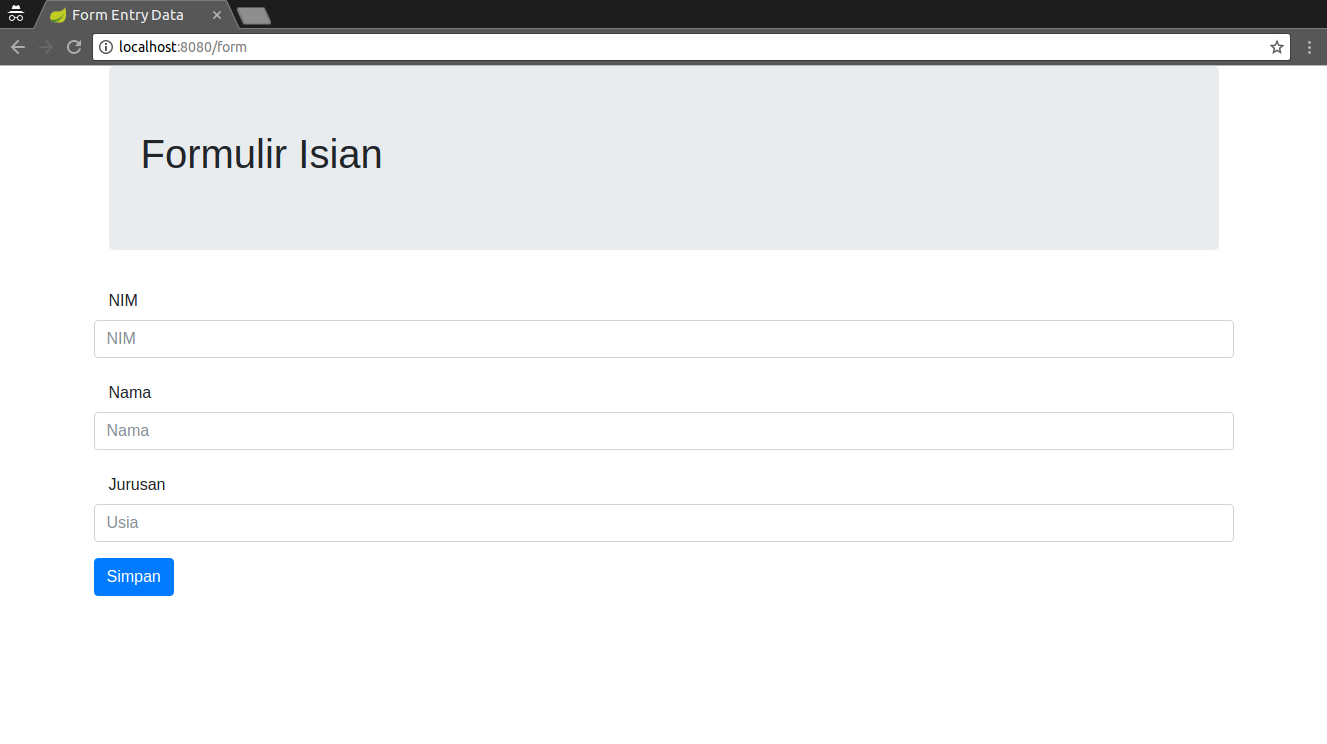
\includegraphics[width=1\textwidth]{./resources/035-halaman-entry-data}
		\caption{Tampilan Halaman \textit{Entry} Data}
		\label{fig:halaman-entry-data}
	\end{figure}
	
	\item Kemudian saat melakukan simpan data, seharusnya datanya tersimpan dan halaman kembali ke \texttt{daftar-mahasiswa} dengan penambahan data dari operasi sebelumnya.
	
\end{enumerate}

Sampai sini usaha kita untuk memberikan fasilitas tambah data selesai.


\section{Ubah Data}

Pada pengubahan data ini, konsepnya adalah menampilkan formulir isian seperti tambah data, hanya saja isian datanya sudah terisi dengan data sebelumnya, \textit{user} atau pengguna hanya mengganti isiannya yang dirasa perlu diperbaiki / diubah, setelah itu melakukan simpan data seperti tambah data dan layar dikembalikan ke \texttt{daftar-mahasiswa} untuk menampilkan hasil perubahaannya. Berikut adalah langkahnya :

\begin{enumerate}
	\item Melakukan perubahan pada halaman \texttt{daftar-mahasiswa} agar memiliki tombol \texttt{Ubah}. Perubahan yang dilakukan pada \textit{file} ini adalah sebagai berikut :
	
	\begin{lstlisting}
<html>
<head>
        <title>Aplikasi Pendataan Mahasiswa</title>
    <link rel="stylesheet" href="https://maxcdn.bootstrapcdn.com/bootstrap/4.0.0-beta.2/css/bootstrap.min.css" integrity="sha384-PsH8R72JQ3SOdhVi3uxftmaW6Vc51MKb0q5P2rRUpPvrszuE4W1povHYgTpBfshb" crossorigin="anonymous"/>
    <script src="https://code.jquery.com/jquery-3.2.1.slim.min.js" integrity="sha384-KJ3o2DKtIkvYIK3UENzmM7KCkRr/rE9/Qpg6aAZGJwFDMVNA/GpGFF93hXpG5KkN" crossorigin="anonymous"></script>
    <script src="https://cdnjs.cloudflare.com/ajax/libs/popper.js/1.12.3/umd/popper.min.js" integrity="sha384-vFJXuSJphROIrBnz7yo7oB41mKfc8JzQZiCq4NCceLEaO4IHwicKwpJf9c9IpFgh" crossorigin="anonymous"></script>
    <script src="https://maxcdn.bootstrapcdn.com/bootstrap/4.0.0-beta.2/js/bootstrap.min.js" integrity="sha384-alpBpkh1PFOepccYVYDB4do5UnbKysX5WZXm3XxPqe5iKTfUKjNkCk9SaVuEZflJ" crossorigin="anonymous"></script>
    <script src="https://ajax.googleapis.com/ajax/libs/angularjs/1.6.6/angular.min.js"></script>
    <script src="/js/app.js"></script>
    <script src="/js/api-controller.js"></script>
</head>
<body ng-app="MahasiswaApp" class="container" >

    <div class="jumbotron">
        <h1>Daftar Mahasiswa</h1>
    </div>

    <div ng-controller="ApiController">

        <table class="table table-striped">
            <thead>
                <tr>
                    <th scope="col">NIM</th>
                    <th scope="col">NAMA</th>
                    <th scope="col">JURUSAN</th>
                </tr>
            </thead>
            <tbody>
                <tr ng-repeat="mhs in daftarMahasiswa">
                    <td>{{mhs.nim}}</td>
                    <td>{{mhs.nama}}</td>
                    <td>{{mhs.jurusan}}</td>
                    (*\textbf{\texttt{<td> }}*)
                      (*\texttt{<button class="btn btn-warning" }*) 
                          (*\texttt{ng-click="ubah(mhs)"> }*)
                        (*\texttt{Ubah}*)
                      (*\texttt{</button> }*)
                    (*\texttt{</td> }*)
                </tr>
            </tbody>            
            <tfoot>
                <tr>
                    <td>
                        <a class="btn btn-primary" href="/form" role="button">Tambah</a>
                    </td>
                </tr>
            </tfoot>
        </table>
    </div>
</body>
</html>
	\end{lstlisting}
	
	Pada baris ke-33 sampai dengan baris ke-38 adalah tambahan kode kita agar nantinya ditiap baris data yang muncul pada \textit{browser} akan muncul pula tombol ubah untuk mengubah data. Perhatikan bahwa pada baris ke-35 ada parameter \texttt{ng-click} yang berisi atau memanggil fungsi \texttt{ubah} yang melewatkan data \texttt{mhs} yang terpilih.
	
	\item Mengubah \textit{file} \texttt{api-controller.js} agar memiliki fungsi \texttt{ubah}. Fungsi \texttt{ubah} ini nantinya hanya melakukan \textit{request} terhadap halaman \texttt{edit-form} dengan disertai parameter \texttt{nim} yang berisi NIM dari data mahasiswa terpilih. Berikut adalah perubahan kode yang kita lakukan terhadap \textit{file} \texttt{api-controller.js} :
	
	\begin{lstlisting}
app.controller('ApiController', function($scope, $http, $window) {
    $scope.daftarMahasiswa = {};
    
    $scope.updateDaftarMahasiswa = function() {
      $http.get('daftar-mahasiswa').then(sukses, gagal);
      //$http.get('daftar-mahasiswa-with-paging').then(sukses, gagal);
      
      function sukses(response) {
          console.log(response);
          $scope.daftarMahasiswa = response.data;
          //console.log(response.data.content);
          //$scope.daftarMahasiswa = response.data.content;
      };
      
      function gagal(response) {
          console.log(response);
      }
    };
    
    (*\texttt{\$scope.ubah = function(mhs) \{ }*)
        (*\texttt{\$window.location.href = 'edit-form?nim=' + mhs.nim; }*)
    (*\texttt{\}; }*)
    
    $scope.updateDaftarMahasiswa();
});
	\end{lstlisting}
	
	Seharusnya nanti halaman yang tampil akan berubah dari \texttt{daftar-mahasiswa.html} menjadi \texttt{edit-form.html}.
	
	\item Langkah berikutnya adalah membuat halaman \texttt{edit-form.html} agar siap menampilkan \textit{response} dari \textit{request} pada langkah sebelumnya. Letak \textit{file} \texttt{edit-form.html} ini sama seperti \textit{file} \texttt{daftar-mahasiswa.html}, berada dalam \textit{folder} \texttt{templates}. Isi kode dari \textit{file} \texttt{edit-form.html} ini adalah seperti berikut :
	
	\begin{lstlisting}
<html>
<head>
    <title>Formulir Ubah Data</title>        
    
    <link rel="stylesheet" href="https://maxcdn.bootstrapcdn.com/bootstrap/4.0.0-beta.2/css/bootstrap.min.css" integrity="sha384-PsH8R72JQ3SOdhVi3uxftmaW6Vc51MKb0q5P2rRUpPvrszuE4W1povHYgTpBfshb" crossorigin="anonymous"/>
    <script src="https://code.jquery.com/jquery-3.2.1.slim.min.js" integrity="sha384-KJ3o2DKtIkvYIK3UENzmM7KCkRr/rE9/Qpg6aAZGJwFDMVNA/GpGFF93hXpG5KkN" crossorigin="anonymous"></script>
    <script src="https://cdnjs.cloudflare.com/ajax/libs/popper.js/1.12.3/umd/popper.min.js" integrity="sha384-vFJXuSJphROIrBnz7yo7oB41mKfc8JzQZiCq4NCceLEaO4IHwicKwpJf9c9IpFgh" crossorigin="anonymous"></script>
    <script src="https://maxcdn.bootstrapcdn.com/bootstrap/4.0.0-beta.2/js/bootstrap.min.js" integrity="sha384-alpBpkh1PFOepccYVYDB4do5UnbKysX5WZXm3XxPqe5iKTfUKjNkCk9SaVuEZflJ" crossorigin="anonymous"></script>
    <script src="https://ajax.googleapis.com/ajax/libs/angularjs/1.6.6/angular.min.js"></script>
    <script src="/js/app.js"></script>
    <script src="/js/edit-form-controller.js"></script>
</head>
<body class="container" ng-app="MahasiswaApp">
    <div class="jumbotron">
        <h1>Formulir Ubah Data</h1>
    </div>
    
    <div ng-controller="EditFormController">
<form>
    <div class="form-group row">
        <label class="col-sm-2 col-form-label">NIM</label>
        <input class="form-control" 
               type="text" 
               placeholder="NIM" 
               ng-model="dataMahasiswa.nim" 
               readonly="true"/>
    </div>
    <div class="form-group row">
        <label class="col-sm-2 col-form-label">Nama</label>
        <input class="form-control" type="text" placeholder="Nama" ng-model="dataMahasiswa.nama"/>
    </div>
    <div class="form-group row">
        <label class="col-sm-2 col-form-label">Jurusan</label>
        <input class="form-control" type="text" placeholder="Usia" ng-model="dataMahasiswa.jurusan" />
    </div>    
    <div class="form-group row">
        <button class="btn btn-primary" ng-click="simpan()">Simpan</button>
    </div>
</form>
    </div>
</body>
</html>
	\end{lstlisting}
	
	Terlihat mirip dengan \textit{file} \texttt{form.html}, namun ada beberapa perbedaan bila kita teliti lebih jauh, perbedaan yang pertama adalah penggunaan \textit{controller} \texttt{EditFormController} seperti disebutkan pada baris ke-18 berikut :
	
	\begin{lstlisting}[firstnumber=18]
	<div ng-controller="EditFormController">\end{lstlisting}
	
	\textit{Controller} ini diambilkan dari \textit{file} \texttt{edit-form-controller.js} seperti terlihat pada baris ke-11 berikut :
	
	\begin{lstlisting}[firstnumber=11]
	<script src="/js/edit-form-controller.js"> \end{lstlisting}
	
	Kemudian menjadikan isian untuk NIM menjadi \textit{read-only} seperti perintah pada baris ke-26 berikut :
	
	\begin{lstlisting}[firstnumber=26]
	readonly="true" /> \end{lstlisting}
	
	\item Membuat \textit{file} \texttt{edit-form-controller.js} agar dapat membaca \textit{url} yang dikirimkan dan mengambil informasi NIM yang terdapat didalamnya. Letak \textit{file} \texttt{edit-form-controller.js} ini sama seperti \textit{controller} lainnya, yaitu berada di \textit{folder} \texttt{static/js/}. Berikut adalah isi kode untuk \textit{file} tersebut :
	
	\begin{lstlisting}
app.controller('EditFormController', function($scope, $window, $http) {
    $scope.dataMahasiswa = {};
    
    $scope.updateData = function() {
        nim = $window.location.search.split('?')[1].split('=')[1];
        $scope.dataMahasiswa.nim = nim;
        $http.get('/get-mahasiswa-by-nim/' + nim).then(sukses, gagal);
        
        function sukses(response) {
            $scope.dataMahasiswa.nama = response.data.nama;
            $scope.dataMahasiswa.jurusan = response.data.jurusan;
        };
        
        function gagal(response) {};
    };
    
    $scope.simpan = function() {
        $http.post('/simpan-edit-data', $scope.dataMahasiswa).then(sukses, gagal);
        
        function sukses(response) {
            $window.location.href = '/';
        };
        
        function gagal(response) {}
    };
    
    $scope.updateData();
});
	\end{lstlisting}
	
	Pada \textit{controller} ini, kita membutuhkan beberapa modul seperti \texttt{\$scope}, \texttt{\$window}, dan \texttt{\$http}. Di dalam \textit{controller} ini, ada objek \texttt{dataMahasiswa} yang fungsinya adalah menyimpan hasil \textit{entry} data pada halaman \texttt{edit-form.html}, kemudian ada sebuah fungsi \texttt{updateData} yang selalu dijalankan apabila \texttt{edit-form} ini dibuka, atau dilakukan \textit{refresh}.
	
	Isi dari fungsi \texttt{updateData} ini yaitu melakukan \textit{parsing} dari \textit{url request} yang terletak di \textit{address browser} seperti pada baris ke-5, kemudian mengisikan parameter \texttt{nim} milik \texttt{dataMahasiswa} agar tampilan \textit{input} di halaman \textit{web} terbarui seperti pada baris ke-6.
	
	Pada baris ke-7 melakukan \textit{request} dengan \textit{method} \texttt{GET} ke \textit{back-end service} dengan sebuah parameter  \texttt{nim}. Apabila berhasil, data \texttt{nama} dan \texttt{jurusan} dari \textit{back-end service} akan ditampilkan dalam komponen yang semestinya.
	
	Pada baris ke-17, kita menyiapkan fungsi \texttt{simpan} yang didalamnya (pada baris ke-18) melakukan \textit{request} data dengan metode \texttt{POST} dengan variabel \texttt{dataMahasiswa} sebagai parameternya.
	
	\item Mengubah kelas \texttt{ApiRestController} agar dapat melakukan respon terhadap \textit{request} \texttt{/get-mahasiswa-by-nim} dengan parameter \texttt{nim}. Isi kode dari kelas \texttt{ApiRestController} adalah seperti berikut ini :
	
	\begin{lstlisting}
package lab.aikibo.cobacrudangular.controller;

import java.util.List;
import lab.aikibo.cobacrudangular.entity.Mahasiswa;
import lab.aikibo.cobacrudangular.repo.MahasiswaRepo;
import lab.aikibo.cobacrudangular.repo.MahasiswaRepoPaging;
import org.springframework.beans.factory.annotation.Autowired;
import org.springframework.data.domain.Page;
import org.springframework.data.domain.Pageable;
import org.springframework.web.bind.annotation.PathVariable;
import org.springframework.web.bind.annotation.RequestBody;
import org.springframework.web.bind.annotation.RequestMapping;
import org.springframework.web.bind.annotation.RequestMethod;
import org.springframework.web.bind.annotation.RestController;

/**
 *
 * @author tamami <tamami.oka@gmail.com>
 */
@RestController
public class ApiRestController {
    
    @Autowired
    private MahasiswaRepo mhsRepo;
    
    @Autowired
    private MahasiswaRepoPaging mhsRepoPaging;
    
    @RequestMapping("/daftar-mahasiswa")
    public List<Mahasiswa> getDaftarMahasiswa() {
        return mhsRepo.findAll();
    }
    
    @RequestMapping("/daftar-mahasiswa-with-paging")
    public Page<Mahasiswa> getDaftarMahasiswaWithPaging(Pageable pageable) {
        return mhsRepoPaging.findAll(pageable);
    }
    
    @RequestMapping(value = "/tambah-data", method = RequestMethod.POST) 
    public void tambahData(@RequestBody Mahasiswa mhs) {
        mhsRepo.save(mhs);
    }    
    
    (*\texttt{@RequestMapping(value = "/get-mahasiswa-by-nim/\{nim\}") }*)
    (*\texttt{public Mahasiswa getMahasiswaByNim( }*)
        (*\texttt{@PathVariable("nim") String nim) \{ }*)
      (*\texttt{return mhsRepo.findOne(nim); }*)
    (*\texttt{\} }*)
    
    (*\texttt{@RequestMapping(value = "/simpan-edit-data", }*)
        (*\texttt{method = RequestMethod.POST) }*)
    (*\texttt{public void simpanEditData(@RequestBody Mahasiswa mhs) \{ }*)
      (*\texttt{mhsRepo.save(mhs); }*)
    (*\texttt{\} }*)
}
	\end{lstlisting}
	
	Pada baris ke-47, kita hanya melihat pemanggilan sebuah fungsi \texttt{findOne} dengan parameter \texttt{nim} yang dipanggil dari \textit{interface repository} yang telah kita buat, yang artinya adalah mengambil sebuah \textit{record} dari bassi data.
	
	Pada baris ke-50 sampai dengan baris ke-54 sebetulnya sama saja dengan \textit{method} \texttt{tambahData} di atasnya, yaitu hanya menyimpan objek Mahasiswa ke dalam sistem basis data.
	
	\item Mendaftarkan \textit{view} \texttt{edit-form} ke Spring MVC pada kelas \texttt{WebConfig} agar dapat dikenali halaman \texttt{edit-form} yang dimaksud, berikut adalah hasil perubahan kode yang terjadi pada \textit{file} \texttt{WebConfig} :
	
	\begin{lstlisting}
package lab.aikibo.cobacrudangular.config;

import org.springframework.context.annotation.Configuration;
import org.springframework.web.servlet.config.annotation.ViewControllerRegistry;
import org.springframework.web.servlet.config.annotation.WebMvcConfigurerAdapter;

@Configuration
public class WebConfig extends WebMvcConfigurerAdapter {

	@Override
	public void addViewControllers(ViewControllerRegistry registry) {
		registry.addViewController("/login").setViewName("login");
		registry.addViewController("/test-angular").setViewName("test-angular");
        registry.addViewController("/").setViewName("daftar-mahasiswa");
        registry.addViewController("/daftar-mahasiswa").setViewName("daftar-mahasiswa");
        registry.addViewController("/form").setViewName("form");
        (*\texttt{registry.addViewController("/edit-form").setViewName("edit-form"); }*)
	}

}
	\end{lstlisting}
	
	\item Mencoba \textit{feature} yang telah jadi. Seharusnya saat dipilihkan tombol \texttt{Ubah} untuk mengubah suatu dari basis data, maka seharusnya akan tampil informasi lengkap data mahasiswa seperti pada gambar \ref{fig:halaman-edit-data} berikut :
	
	\begin{figure}[H]
		\centering
		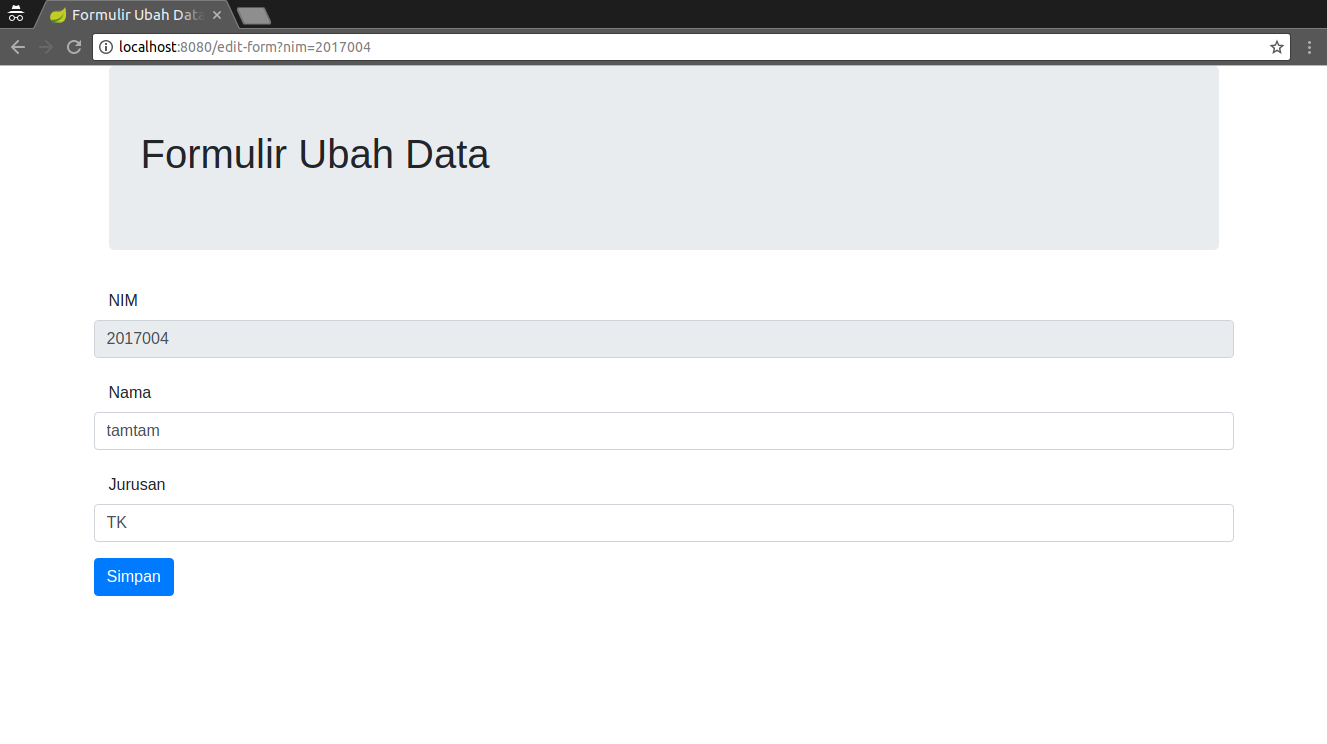
\includegraphics[width=1.0\textwidth]{./resources/036-tampilan-edit-form}
		\caption{Halaman Untuk \texttt{edit-form.html}}
		\label{fig:halaman-edit-data}
	\end{figure}
	
	Sampai sini, apabila tombol disimpan maka halaman akan kembali ke \texttt{daftar-mahasiswa} dengan menyertakan hasil perubahannya.
\end{enumerate}
	

\section{Hapus Data}

Kali ini kita akan menambahkan fasilitas untuk melakukan hapus data, skenarionya akan mirip dengan \textit{edit} data, dimana nanti dari daftar mahasiswa, akan dilakukan \textit{request} dengan parameter NIM. Berikut langkah kodenya :

\begin{enumerate}
	\item Mengubah / menambahkan tombol \texttt{Hapus} di \textit{file} \texttt{daftar-mahasiswa.html}. Perubahan kode yang dilakukan adalah sebagai berikut :
	
	\begin{lstlisting}
<html>
<head>
        <title>Aplikasi Pendataan Mahasiswa</title>
    <link rel="stylesheet" href="https://maxcdn.bootstrapcdn.com/bootstrap/4.0.0-beta.2/css/bootstrap.min.css" integrity="sha384-PsH8R72JQ3SOdhVi3uxftmaW6Vc51MKb0q5P2rRUpPvrszuE4W1povHYgTpBfshb" crossorigin="anonymous"/>
    <script src="https://code.jquery.com/jquery-3.2.1.slim.min.js" integrity="sha384-KJ3o2DKtIkvYIK3UENzmM7KCkRr/rE9/Qpg6aAZGJwFDMVNA/GpGFF93hXpG5KkN" crossorigin="anonymous"></script>
    <script src="https://cdnjs.cloudflare.com/ajax/libs/popper.js/1.12.3/umd/popper.min.js" integrity="sha384-vFJXuSJphROIrBnz7yo7oB41mKfc8JzQZiCq4NCceLEaO4IHwicKwpJf9c9IpFgh" crossorigin="anonymous"></script>
    <script src="https://maxcdn.bootstrapcdn.com/bootstrap/4.0.0-beta.2/js/bootstrap.min.js" integrity="sha384-alpBpkh1PFOepccYVYDB4do5UnbKysX5WZXm3XxPqe5iKTfUKjNkCk9SaVuEZflJ" crossorigin="anonymous"></script>
    <script src="https://ajax.googleapis.com/ajax/libs/angularjs/1.6.6/angular.min.js"></script>
    <script src="/js/app.js"></script>
    <script src="/js/api-controller.js"></script>
</head>
<body ng-app="MahasiswaApp" class="container" >

    <div class="jumbotron">
        <h1>Daftar Mahasiswa</h1>
    </div>

    <div ng-controller="ApiController">

        <table class="table table-striped">
            <thead>
                <tr>
                    <th scope="col">NIM</th>
                    <th scope="col">NAMA</th>
                    <th scope="col">JURUSAN</th>
                </tr>
            </thead>
            <tbody>
                <tr ng-repeat="mhs in daftarMahasiswa">
                    <td>{{mhs.nim}}</td>
                    <td>{{mhs.nama}}</td>
                    <td>{{mhs.jurusan}}</td>
                    <td>
                        <button class="btn btn-warning" ng-click="ubah(mhs)">
                            Ubah
                        </button>
                    </td>
                    (*\texttt{<td> }*)
                      (*\texttt{<button class="btn btn-danger" }*)
                          (*\texttt{ng-click="hapus(mhs)"> }*)
                        (*\texttt{Hapus }*)
                      (*\texttt{</button> }*)
                    (*\texttt{</td> }*)
                </tr>
            </tbody>            
            <tfoot>
                <tr>
                    <td>
                        <a class="btn btn-primary" href="/form" role="button">Tambah</a>
                    </td>
                </tr>
            </tfoot>
        </table>
    </div>
</body>
</html>
	\end{lstlisting}
	
	Pada baris ke-40, ada parameter \texttt{ng-click} yang akan memanggil fungsi \texttt{hapus} dengan parameter \texttt{mhs} yang terpilih.
	
	\item Merubah \textit{file} \texttt{api-controller.js} agar memiliki fungsi \texttt{hapus}. Berikut adalah perubahan atau penambahan kode yang terjadi di \textit{file} \texttt{api-controller.js} :
	
	\begin{lstlisting}
app.controller('ApiController', function($scope, $http, $window) {
    $scope.daftarMahasiswa = {};
    
    $scope.updateDaftarMahasiswa = function() {
      $http.get('daftar-mahasiswa').then(sukses, gagal);
      //$http.get('daftar-mahasiswa-with-paging').then(sukses, gagal);
      
      function sukses(response) {
          console.log(response);
          $scope.daftarMahasiswa = response.data;
          //console.log(response.data.content);
          //$scope.daftarMahasiswa = response.data.content;
      };
      
      function gagal(response) {
          console.log(response);
      }
    };
    
    $scope.ubah = function(mhs) {
        $window.location.href = 'edit-form?nim=' + mhs.nim;
    };
    
    (*\texttt{\$scope.hapus = function(mhs) \{ }*)
        (*\texttt{\$http.delete('/hapus/' + mhs.nim).then(sukses, gagal); }*)
        
        (*\texttt{function sukses(response) \{ }*)
            (*\texttt{\$scope.updateDaftarMahasiswa(); }*)
        (*\texttt{\}; }*)
        
        (*\texttt{function gagal(response) \{\} }*)
    (*\texttt{\}; }*)
    
    $scope.updateDaftarMahasiswa();
});
	\end{lstlisting}
	
	\item Merubah kelas \texttt{ApiRestController} agar dapat melakukan \textit{response} terhadap \textit{request} \texttt{/hapus/\{nim\}}. Perubahan yang kita lakukan adalah sebagai berikut :
	
	\begin{lstlisting}
package lab.aikibo.cobacrudangular.controller;

import java.util.List;
import lab.aikibo.cobacrudangular.entity.Mahasiswa;
import lab.aikibo.cobacrudangular.repo.MahasiswaRepo;
import lab.aikibo.cobacrudangular.repo.MahasiswaRepoPaging;
import org.springframework.beans.factory.annotation.Autowired;
import org.springframework.data.domain.Page;
import org.springframework.data.domain.Pageable;
import org.springframework.web.bind.annotation.PathVariable;
import org.springframework.web.bind.annotation.RequestBody;
import org.springframework.web.bind.annotation.RequestMapping;
import org.springframework.web.bind.annotation.RequestMethod;
import org.springframework.web.bind.annotation.RestController;

/**
 *
 * @author tamami <tamami.oka@gmail.com>
 */
@RestController
public class ApiRestController {
    
    @Autowired
    private MahasiswaRepo mhsRepo;
    
    @Autowired
    private MahasiswaRepoPaging mhsRepoPaging;
    
    @RequestMapping("/daftar-mahasiswa")
    public List<Mahasiswa> getDaftarMahasiswa() {
        return mhsRepo.findAll();
    }
    
    @RequestMapping("/daftar-mahasiswa-with-paging")
    public Page<Mahasiswa> getDaftarMahasiswaWithPaging(Pageable pageable) {
        return mhsRepoPaging.findAll(pageable);
    }
    
    @RequestMapping(value = "/tambah-data", method = RequestMethod.POST) 
    public void tambahData(@RequestBody Mahasiswa mhs) {
        mhsRepo.save(mhs);
    }    
    
    @RequestMapping(value = "/get-mahasiswa-by-nim/{nim}")
    public Mahasiswa getMahasiswaByNim(@PathVariable("nim") String nim) {
        return mhsRepo.findOne(nim);
    }
    
    @RequestMapping(value = "/simpan-edit-data", method = RequestMethod.POST)
    public void simpanEditData(@RequestBody Mahasiswa mhs) {
        mhsRepo.save(mhs);
    }
    
    (*\texttt{@RequestMapping(value = "/hapus/{nim}", }*)
        (*\texttt{method = RequestMethod.DELETE) }*)
    (*\texttt{public void deleteData(@PathVariable("nim") String nim) \{ }*)
      (*\texttt{mhsRepo.delete(nim); }*)
    (*\texttt{\} }*)
}
	\end{lstlisting}
	
	\item Melakukan uji coba. Gambar \ref{fig:halaman-dengan-hapus-data} adalah hasil tampilan dari aplikasi yang telah memiliki fasilitas untuk hapus data :
	
	\begin{figure}[H]
		\centering
		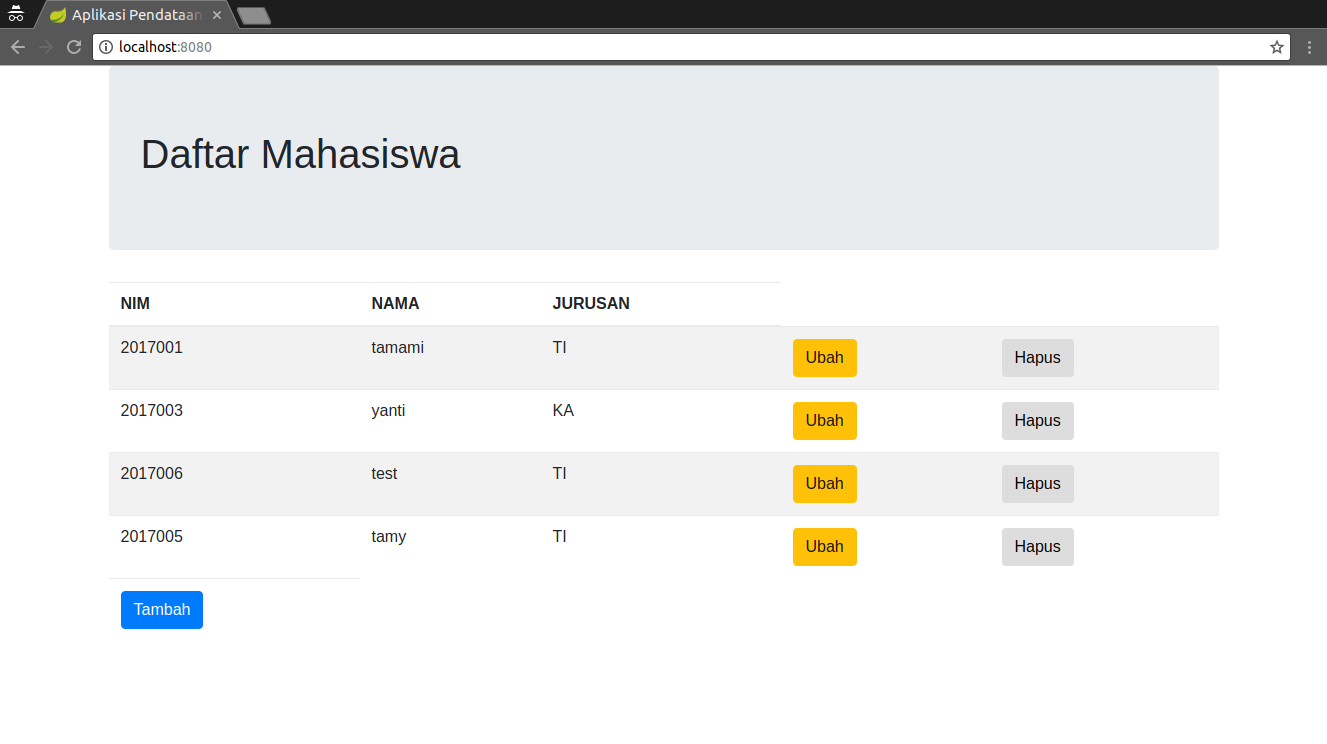
\includegraphics[width=1\textwidth]{./resources/037-halaman-dengan-hapus-data}
		\caption{Halaman Daftar Mahasiswa Dengan Fasilitas Hapus Data}
		\label{fig:halaman-dengan-hapus-data}
	\end{figure}
	
\end{enumerate}

Sampai sini aplikasi \textit{web} yang telah kita bangun memiliki fasilitas yang lengkap yang terdiri dari penambahan data, pengubahan data, dan penghapusan data.